% The current problem is sudo apt-get install texlive-fonts-extra

\documentclass[11pt]{scrartcl}
\usepackage[sexy]{evan}
% \usepackage{multirow}
\usepackage{array}
% \usepackage{program}
\usepackage{algorithm}
\usepackage{algpseudocode}
\usepackage{bbm}
\begin{document}

\title{Mathematics of Machine Learning}
\author{Arthur Conmy\footnote{Please send any corrections and/or feedback to \url{asc70@cam.ac.uk}}}
\date{Part II, Lent Term 2021}

\maketitle
\begin{abstract}
These notes are based on lectures given (virtually) by Dr R. Shah in Lent term 2021. 
Credit is also due to Evan Chen for the style file for these notes\footnote{Available here: \url{https://github.com/vEnhance/dotfiles/blob/master/texmf/tex/latex/evan/evan.sty}.}.
\end{abstract}

\tableofcontents

\section{Introduction}

The course will be divided into three parts:

\begin{itemize}
    \item Statistical learning theory (including empirical risk minimization).
    \item Computation (including (stochastic) gradient descent).
    \item Popular methods in practise.
\end{itemize}

The course will move from a more theoretical background to practical things. There is a significant gap between the theory and the practise in machine learning, as will be seen in the course.

% The most important prerequisite is 1A Probability. IB Optimization, IB Analysis and Topology and IB Statistics provide some background, though only in parts (e.g. convex optimization, cts functions attaining their bounds on closed bounded sets and linear regression for building intuition).

% The course web 

% \section{Lecture 1}

\subsection{Conditional Expectation}

The results stated here are true subject to certain convergence conditions. II Stochastic Financial Models and II Probability and Measure deal with such things more formally. For our purposes, we will use the results as tools to develop theory.

% Much of this setup is from 1A Probability:

\begin{definition}
[Conditional density]
Let $Z$ and $W$ be random variables with joint density $f(z,w)$, and let $f_W(w)$ be the marginal density of $W$ (integrate over all $z$ values). Then the \vocab{conditional density} of $z$ given $w$ is

% \begin{equation}
%     f_{Z\mid W}(z,w) = \begin{cases}
%       f(z,w) / f_W(w) & \text{where $f_W(w) \neq 0$.} \\
%       0 & \text{otherwise.}
%     \end{cases}
% \end{equation}
% \end{definition}

% \begin{definition}
[Conditional expectation]
In the same notation as above, we define the \emph{random variable} $\E{Z\mid W}$ as

\begin{equation}
    \E{Z\mid W} = \int z f_{Z\mid W}(z,W) \mathrm{d}z.
\end{equation}
\end{definition}

Note that $\E{Z\mid W}$ is a function of a random variable ($W$), so is itself a random variable. It is not simply a number, as ordinary expectations are. 

\begin{remark}
[Digression: design choice]
I have reorganised this section to include condtional expectation things before the initial setup for ERM.This is because I have found conditional expectation one of the most frustrating (though certainly necessary) parts of the course, so any familiarity now will help later, but total familiarity is probably not to be expected.
\end{remark}

\begin{remark}We can interpret $\E{Z|W}$ as `the function of $W$ that's our best guess for $Z$ given only the information contained in $W$'\footnote{see \url{https://dynalist.io/d/bx3GM7El5D_PsHTOvxgJlTyW}}.
\label{neels remark}
\end{remark} 

\begin{remark}
In this course, whenever we are conditioning over something, think of this as what is currently fixed.

Two examples from later in the course are in the definition of risk (\ref{L1:Risk Definition}), we've chosen our hypothesis $h$ and are now evaluating the expectation of the loss (risk); we are NOT considering some non-deterministic method for generating $h$ for example

This is perhaps counterintuitive since of course $\E{Z|W}$ is a random \textit{variable} that's a function of $W$ however ...
\end{remark}

Interpretation (\ref{neels remark}) gives some intuition behind the next result, which generalises what we did in IA.

\begin{theorem}
[General tower property]
Let $f : \mathbb{R}^d \rightarrow \mathbb{R}^m$ and $Z$ and $W$ be random variables. Then 

\begin{equation}
\mathbb{E}[\mathbb{E}[Z\mid W]\mid f(W)] = \mathbb{E}[Z\mid f(W)].
\end{equation}
\end{theorem}

\begin{theorem}
[Taking out what is known]
Let $f$ be real-valued. Then

\begin{equation}
    \mathbb{E}[f(W)Z\mid W) = f(W)\mathbb{E}[Z\mid W].
\end{equation}
\label{L1: Taking out}
\end{theorem}

As an example of how to use these tools,

\begin{theorem}
[Best least squares predictor]
\label{best least squares}

The following holds:

\begin{equation}
    \E{Z-f(W)}^2 = \E{Z - \E{Z \mid W}}^2 + \E{f(W)-\E{Z \mid W}}^2.
\end{equation}

We will write out the extended details of how to apply our conditional expectation theory to get this result.

\begin{proof}
Initially, add the obvious term to the LHS:

\begin{align*}
    \E{Z-f(W)}^2 = \E{Z-\E{Z\mid W} + \E{Z\mid W} - f(W)}^2 \\
    = \E{Z - \E{Z \mid W}}^2 + \E{f(W)-\E{Z \mid W}}^2 \\
    - 2 \E{Z - \E{Z\mid W}} \E{f(W)-\E{Z\mid W}}.
\end{align*}

So we need to show that $\E{Z - \E{Z\mid W}} \E{f(W)-\E{Z\mid W}}=0$.

We do this by using the tower property to insert a condition on $W$:

\begin{align*}
    \E{Z - \E{Z\mid W}} \E{f(W)-\E{Z\mid W}} \\
    = \E{ \E{Z - \E{Z\mid W}} \E{f(W)-\E{Z\mid W}} \mid W}.
\end{align*}

From here we can pull out the latter expectation term, since it's a function of $W$, by (\ref{L1: Taking out}). The former term left inside the expectation is 0, since

\begin{align*}
    \E{Z - \E{Z \mid W} \mid W} = \E{Z \mid W} - \E{\E{Z \mid W} \mid W} \\
    = \E{Z \mid W} - \E{Z \mid W} = 0
\end{align*}

using the tower property once more.

\end{proof}
\end{theorem}

We'll introduce terminology in the next section that means that this result is saying that the hypothesis $h:\mathcal{X} \rightarrow \mathbb{R}$ minimising $R(h)$ under squared error loss is $h_0(x)=\E{Y \mid X = x}$, and nothing deeper than this (by considering $Z=Y$ and $X=W$).

\begin{theorem}
[Conditional Jensen]
Given convex $f:\RR \rightarrow \RR$,

\begin{equation}
    \E{f(Z) \mid W} \ge f(\E{Z|W}).
\end{equation}
\end{theorem}

\begin{remark}
To remember which way round Jensen's inequality goes (keeping $W$ constant) choose $f(x)=x^2$, and use that variance is non-negative.
\end{remark}

The proof is in two parts. Both are not examinable, but while the full proof uses II Probability and Measure and is outside the scope of the course, the lemma is an idea from IA Probability that we will see used on several occasions in this course.

\begin{lemma}
Suppose that $f : \RR \to \RR$ is convex. Then $\forall x \in \mathbb{ R}$, if 

\begin{equation}
\partial f(x) := \{ g : f(z) \ge (z-x)g + f(x) \}
\end{equation}

then 
\begin{enumerate}
\item $\partial f(x) = [a, b]$ where $a \le b \in \mathbb{ R}$.
\item \begin{equation}
    a = \lim_{\varepsilon \downarrow 0} \frac{f(x+\varepsilon ) - f(x)}{\varepsilon }
\end{equation}
and 
\begin{equation}
    b = \lim_{\varepsilon \downarrow 0} \frac{f(x) - f(x-\varepsilon )}{\varepsilon }.   
\end{equation}
\end{enumerate}

\begin{proof}(Sketch)
We will later interpret $\partial f(x)$ as the set of \textit{subgradients} at $x$, see (\ref{subgradient_section}).

For 1), after drawing a picture of a convex function this should be clear. One sketch proof is to consider $[a_0, b_0]$, where $a_0 = f(x) - f(x-1)$ and $b_0 = f(x+1) - f(x)$. Then either these already work, or WLOG $b_0$ fails because there's some $y \in (x, x+1)$ below the line through $(x,f(x))$ with gradient $b_0$. But by convexity this line will have no points $(z, f(z))$ below it where $z<x$. Similarly the equivalent $a_0$ line won't have points below it where $z>x$. So increasing $a_0$ and decreasing $b_0$ must lead to an interval $[a,b]$, because at some point we must `cross over' from points lying below on the left to points lying below on the right, and moreover by continuity we must get $[a,b]$ non-empty since there can't be failures on both sides.

For 2), suppose not, then argue by convexity that actually there must be points closer to $x$ with gradient closer to $a$ and $b$.
\end{proof}
\end{lemma}

\begin{proof}(Conditional Jensen)
See [4], Theorem 23.9. The entire PDF is recommended for a very good formalisation of conditional probability.
\end{proof}

\subsection{Terminology}

We will set up definitions in order to solve classification problems like MNIST or spam detection.

Consider a pair of random variables $(X, Y) \in \mathcal{X} \times \mathcal{Y}$ with joint distribution $P_0$. We call $X$ the \vocab{input} or \vocab{predictor} and $Y$ the \vocab{output} or \vocab{response}.

Our goal is to predict $Y$ from $X$. We do this via a \vocab{hypothesis}\footnote{the use of the term is unlike the use in `hypothesis testing' from statistics.} $h: \mathcal{X} \rightarrow \mathcal{Y}$, and measure the quality of the prediction using a \vocab{loss function} $\ell : \mathcal{Y} \times \mathcal{Y} \rightarrow \mathbb{R}$.

We can be in the \vocab{classification} setting where $\mathcal{Y} = \{ -1, 1 \}$, and typically $\ell$ is the \vocab{misclassification loss}, or `0-1 loss' $\ell (h(x), y) = \one{h(x) \neq y}$. Here, we refer to $h$ as a \vocab{classifier}.

Alternatively, we can be in the \vocab{regression} setting, where $\mathcal{Y} = \mathbb{R}$ and typically $\ell$ is the squared error: $\ell(h(x), y) = (h(x) - y)^2$.

Our aim is to pick $h$ with small \vocab{risk}

\begin{equation}
    R(h) = \mathbb{E}[\ell(h(X), Y) \mid h].
    \label{L1:Risk Definition}
\end{equation}

We have the conditioning over $h$ as we consider the classifier to be fixed; $h$ will be generally constructed from some random data, and this takes that into account. % I think this is related to the fact that we only care about model performance on test data, not training data.

A classifier $h_0$ that minimises the 0-1 risk is called a \vocab{Bayes classifier}. Its associated risk is the \vocab{Bayes risk}.

Define the \vocab{regression function} $\eta$ as 

\begin{equation}
    \eta(x) = \mathbb{P}(Y=1\mid X=x).
    \label{L1:Regression Function}
\end{equation}

Note that in practise we don't have `access' to $\eta$, since to know $\eta$ we need to know the joint distribution to evaluate it; Bayes risk essentially minimises \textit{population-wide} risk. We'll go on to study empiricial risk minimisation (ERM), where we minimise risk with respect to our `training data' (a finite sample of data that we observe empirically).

\begin{theorem}
\label{not deep Bayes}
A Bayes Classifier is given by 

\begin{equation}
    h_0(x) = 
    \begin{cases} 
      1 & \text{if $\eta(x) > 1/2$} \\
      -1 & \text{otherwise.}
   \end{cases}
\label{L1:Bayes Example}
\end{equation}

\begin{proof}
This is not a deep result. The 0-1 risk is just the dumb function `0 if we were right, 1 if we were wrong' so the risk, given $X=x$ is

\begin{align*}
    R(h(x)) = \one{h(x) = 1} \P{Y = -1 \mid X = x} + \one{h(x) = -1} \P{Y = 1 \mid X = x} \\
    = \one{h(x) = 1} (1 - \eta(x)) + \one{h(x) = -1} \eta(x).
\end{align*}

Now we want to minimise this, so just do casework on $\eta(x) < \frac12$, $\eta(x) = \frac12$ and $\eta(x) > \frac12$. In each case our Bayes classifier will be optimal.
% \ell(y_1', \tilde{h}(x_1'))
\end{proof}

\end{theorem}

In reality, we have \vocab{training data} that is a set of iid copies $(X_1, Y_1)$, $(X_2, Y_2)$, $\cdots$, $(X_n, Y_n)$ of $(X, Y)$. We want to use this to construct $\hat{h}$ minimising $R(\hat{h})$. Therefore the conditioning in (\ref{L1:Risk Definition}) will be on this training data, when considering $R(\hat{h})$.

The classical statistical approach is to model $P_0$ using a parametric family. In this approach, we need estimate these unknown parameters.

The machine learning approach is that we're given a class $\H$ from which we will then pick $\hat{h}$. In this approach, we will need an algorithm for picking $\hat{h}$.

\begin{definition}
[Sign]

$\sgn$ is the sign ($\pm1$) of a real, and we define $\text{sgn}(0)=-1$ in this course.

For this reason, in the two-class classification problem, we will label the classes with $+1$ and $-1$ rather than 0 and 1, as seen elsewhere.
\end{definition}

\begin{example}[Examples of $\H$]
\begin{equation}
    \H = \{ x \mapsto \text{sgn} (\mu + x^T \beta) \}
    \label{L1:NN H Class}
\end{equation}

where $\mu \in \mathbb{R}$ and $\beta \in \mathbb{R}^p$ is one example of a class. Another is

\begin{equation}
    \H = \left\{ x \mapsto \text{sgn} \left( \sum_{j}
     \phi_j(x) w_j \right) \right\}
    \label{L1:NN H Class Phi}
\end{equation}

where $w \in \mathbb{R}^d$ and $\phi_j \in \mathbb{B}$ for a given class of functions $\mathbb{B} = \{ f : \mathcal{X} \rightarrow \mathbb{R} \}$. Note that these classes have, in general, many degrees of freedom.
\end{example}

% \section{Lecture 2}

\section{Statistical Learning Theory}
% \section{Empricial Risk Minimisation (ERM)}

As alluded to earlier, minimising population-wide risk is generally not practical nor possible when applying ML methods. So almost all ML methods aim to minimise \vocab{empirical risk}: %So we concern ourselves solely with the training data:

\begin{definition}[Empirical Risk]
Empirical risk or \vocab{training error} is the expectation of the loss $\ell (h(X), Y)$ where $(X,Y)$ follows the \textit{empirical} distribution (which will generally (always?) be some number of iid samples from $P_0$):

\begin{equation}
    \hat{R}(h) = \frac1n \sum_i \ell (h(X_i), Y_i)
\label{L2:ER}
\end{equation}
\end{definition}

Given some class $\H$ of hypotheses, the argmin over this set with respect to this empirical risk is called the empirical risk minimiser.

We've used a lot of words, but there are immediate examples that this setup allows us to describe:

\begin{example}
[Least squares regression from IB Statistics]

In this familiar setting, our class of hypotheses is

\begin{equation}
    \H = \{ x \mapsto (\mu + x^T \beta) \}
\label{L2:Linear Regression H}
\end{equation}

where $\mu \in \mathbb{R}$ and $\beta \in \mathbb{R}^p$, and our loss function is squared error

\begin{equation}
    \ell(X_i,Y_i) = (Y_i - \mu - X_i^T \beta)^2.
\end{equation}
\end{example}

\begin{example}
% [Dividing points by hyperplanes]
[0-1 classification]

If $\mathcal{Y}= \{ -1, +1 \}$, $\H = \{ x \mapsto \sgn{\mu + x^T \beta} \}$ (see (\ref{L1:NN H Class})) and our loss is 0-1 loss, then what we're doing here is finding a hyperplane that divides space into two regions, one for each of -1 and 1, and the empirical loss will be the number of 1s in the -1 region plus the number of -1s in the 1 region, all over $n$. Visually:

\begin{center}              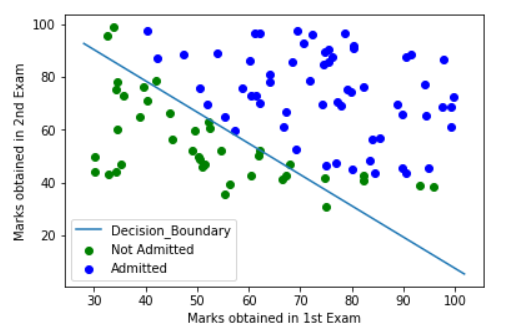
\includegraphics[scale=0.5]{decisionboundary.png}
    \label{fig:L2 Decision Boundary}
\end{center}

The hyperplane in this case is known as the \emph{decision boundary}.
\end{example}

\begin{definition}
[Aitch, aitch and aitch]

Let $\hat{h} \in \H$ be the hypothesis minimising empirical risk.

Let $h^* \in \H$ be the hypothesis minimising (population) risk over all $\H$.

Let $h_0$ be the function minimising (population) risk over all functions $h : \mathcal{X} \to \mathcal{Y}$.
\end{definition}

Note that $h_0$, the `God hypothesis' won't be a perfect predictor, since our data comes from $P_0$, an inherently random distribution. 
We can now consider

\begin{equation}
    R(\hat{h}) - R(h_0) = \underbrace{R(\hat{h}) - R(h^*)}_{\text{\textbf{Excess risk} from our}\atop \text{choice within hypothesis class.}} + \underbrace{R(h^*) - R(h_0)} _{\text{\textbf{Appoximation error} from our} \atop \text{choice of hypothesis class.}}
\label{L2:excess risk and approx error}
\end{equation}

where the terms have the given interpretations. Furthermore, the first term can be seen as a measure of how much we overfit to the training data, and the latter term how much we underfit the underlying distribution by choosing too restrictive a $\H$.

% We are going to be occupied with minimising the excess risk, making statements such as

% \begin{quote}
%     `with probability at least $1-\delta$, $R(\hat{h}) - R(h_0) \le \eps$'
% \end{quote}

% for $\eps$ a function of both $\delta$ and the complexity of $\H$.

Write 

\begin{align}
    R(\hat{h}) - R(h^*) = R(\hat{h}) - \hat{R}(\hat{h}) + \underbrace{\hat{R}(\hat{h}) - \hat{R}(h^*)}_{\le 0} + \hat{R}(h^*) - R(h^*) \\
    \le R(\hat{h}) - \hat{R}(\hat{h}) + \hat{R}(h^*) - R(h^*).
\label{FineForFinite}
\end{align}

where the middle term is non-positive since we chose $\hat{h}$ to be optimal on the training data.

We've interpreted all these terms already, except $\hat{R}(h^*)$. This is the risk of the optimal classifier with respect to all $\H$, but when it can only see the training data. So $\hat{R}(h^*) - R(h^*)$ is another measure of how much we are overfitting.

\subsection{Sub-Gaussianity and Hoeffding's Inequality}

Recall Markov's inequality from IA Probability. Note that this is a simple inequality, but has a nice consequence (on an example sheet from that course).

\begin{theorem}
[Chernoff Bound]
Let $W$ be a random variable and $\alpha > 0$. Then
\begin{equation}
    \P{W \ge t} \le e^{- \alpha t} \E{e^{\alpha W}}
\label{L2 Chernoff}
\end{equation}

\begin{proof}
% Markov's inequality is that $\P{X \ge a} \le \frac1a \E{X}$.

For any increasing function $\phi : \RR \rightarrow [0, \infty)$, $W \ge t$ implies $\phi(W) \ge \phi(t)$, so in this case

\begin{equation}
    \P{W \ge t} \le \P{e^{\alpha W} \ge e^{\alpha t}} \le e^{- \alpha t} \E{e^{\alpha W}}
\end{equation}

by Markov's inequality, as required.
\end{proof}
\end{theorem}

This is important since this has introduced an MGF.

\begin{example}
[A tail bound for Gaussian random variables]
Suppose $W \sim N(0,\sigma^2)$, so has MGF $\E{e^{\alpha W}} = \exp{\frac12 \alpha^2 \sigma^2}$. Then for $t>0$,

\begin{equation}
    \P{W \ge t} \le \exp{-\alpha t + \frac12 \alpha^2 \sigma^2}.
\label{L2:Gaussian tail bound}
\end{equation}

Taking the infinimum over all $\alpha > 0$, we get 

\begin{equation}
    \P{W \ge t} \le \exp{-t/2\sigma^2}.
\label{L2:Gaussian tail bound 2}
\end{equation}
\end{example}

This derivation essentially uses bounding with MGFs. This motivates

\begin{definition}
[Sub-Gaussian]
A random variable $W$ is \vocab{sub-Gaussian} with parameter $\sigma > 0$ if

\begin{equation}
    \E{\exp{\alpha(W - \E{W}}} \le \exp{\frac12 \alpha^2 \sigma^2}
\end{equation}

for every $\alpha \in \RR$.
\end{definition}

i.e. after normalising to mean 0, the MGF of $W$ is always less than the MGF of a variance $N(0,\sigma^2)$ random variable.

\begin{example}
[Basic properties of sub-Gaussian random variables]
Let $W$ be a sub-Gaussian random variable with parameter $\sigma>0$. Then
\begin{itemize}
    \item $W$ is sub-Gaussian for all $\sigma' \ge \sigma$.
    \item $-W$ is also sub-Gaussian.
    \item $\P{W - \E{W} \ge t} \le \exp{-t^2 / 2 \sigma^2}$.
    \item $\P{| W - \E{W}| \ge t} \le 2\exp{-t^2 / 2 \sigma^2}$
\end{itemize}

\label{L2: subg properties}

\begin{proof}
The first two remarks are immediate. To see the third, apply the Chernoff bound since it directly introduces an MGF. The fourth is then a corollary of the third, using the second.

The third property is called the \emph{sub-Gaussian tail bound}, and we will repeatedly use it.
\end{proof}
\end{example}

\begin{definition}
A \emph{Rademacher random variable} $\eps$ takes values $\pm 1$ with equal probability.
\end{definition}

\begin{theorem}
A Rademacher random variable is sub-Gaussian with $\sigma=1$.

\begin{proof}
Directly compute

\begin{align*}
    \E{e^{\alpha \eps}} = \frac12(e^\alpha + e^{-\alpha}) = \sum_{k=0}^{\infty} \frac{\alpha^{2k}}{(2k)!} \\
    \le \sum_{k=0}^{\infty} \left(\frac{\alpha^2}{2} \right)^k \frac{1}{k!} \\
    = e^{\alpha^2 / 2}.
\end{align*}
\end{proof}
\end{theorem}

%lecture 3

How does this relate to ERM? This brings us onto the first deeper result of the course.

\begin{theorem}
[Hoeffding's Lemma]
If $W$ takes values in an interval $[a,b]$, then $W$ is sub-Gaussian with parameter $(b-a)/2$.
\end{theorem}

We will mention three proofs. The first is direct and elementary (from \cite{HoeffdingExercise}). The second (lectured) will prove the weaker result with $\sigma = b-a$, using a technique called \emph{symmetrisation} which will use again later. On the example sheet, a \emph{change of measure} argument\footnote{see \cite{MIT Notes}, also.} is used to prove the full result.

\begin{proof}[Proof 1: elementary]
It suffices to prove the result for $W$ with values in $[0,1]$.

We can directly show that $\E{e^{\alpha(W - \E{W})}} \le e^{-\alpha \E{W}} ( \E{W}(e^\alpha -1) + 1 )$ by Taylor expansion, and then verify that that RHS expression is at most $e^{\frac18 \alpha^2}$ for all $\alpha$, which is sufficient.
\end{proof}

\begin{proof}[Proof 2: symmetrisation]
To check whether a random variable is sub-Gaussian we normalize so the mean is zero, so WLOG assume $\E{W}=0$.

We want to use the results already established for Rademacher random variables, and to do this we cook up $W'$ an independent copy of $W$ so that the random variable $W-W'$ is symmetric about 0, meaning that $\eps (W - W')$ and $W - W'$ have the same distribution (written $W - W' \deq \eps(W - W')$). We write %and then we could consider %In this case, $W \deq \eps W$ where $\eps$ is a Rademacher random variable that's independent of $W$. Moreover, conditional expectations can be thought of as `fixing' the variable conditioned on, so actually 

\begin{equation}
    \E{e^{\alpha \eps (W-W')} \mid W, W'} \le \exp{\alpha (W-W')^2 / 2} \le \exp{\alpha^2 (b-a)^2 / 8},
\label{L3 ideal Hoeffding}
\end{equation}

where conditioning on $W, W'$ effectively fixes these random variables, allowing us to use the Rademacher result.

% % if we supposed that $|X|$ was at most $b-a$ (the use of $a$ and $b$ is not accidental!).

% Now $W-W'$ \emph{is} symmetric about 0, where $W'$ is an independent copy of $W$.

% So now if we can show that 

% \begin{equation}
%     \E{e^{\alpha \eps W} | W, W'} \le \E{e^{\alpha \eps (W-W')} | W, W'}
% \end{equation}

% we get the result. But this is obvious, since the right hand side factors due to the independence of $W$ and $W'$, and then we can use Jensen to show $\E{\exp{- \alpha W'}} \ge $

% The first new random variable we'll introduce is an independent copy $W'$ of $W$. Then assuming we can generalise normal linearity of expectation to the conditional case, i.e. that

We relate this back to $W$ by noting that the familiar linearity of expectation property

\begin{equation}
    \E{X + Y \mid Z} = \E{X \mid Z} + \E{Y \mid Z}
\end{equation}

(where all the expectations are defined) holds, so we have that 

\begin{equation}
    \alpha (W - \E{W}) = \E{\alpha(W-W') \mid W}.
\end{equation}

Therefore

\begin{align}
    \E{\exp{\alpha W}} = \E{\exp{\alpha (W-\E{W'})}} \\
    = \E{\exp{\E{\alpha(W-W') \mid W}}} \\
    \le \E{\exp{\alpha (W-W')}}. %todo decide what to do about equation numbers
\end{align}

where in the last step we apply conditional Jensen, and then simplify via the tower property in the degenerate case conditioning on some constant random variable, to go from to expectation signs to just one.

Finally, we can use the tower property once more to write the equality

\begin{equation}
    \E{\exp{\alpha (W-W')}} = \E{\E{ \exp{\alpha \eps (W-W')} \mid W, W' }}
\end{equation}

where to be specific, we choose the $f$ in the tower property statement to be some degenerate (e.g constant) function to complete the argument (in essence we omit something like `... $\mid 42]$' at the end of both of the above expectation expressions). We've recovered (\ref{L3 ideal Hoeffding}), so we're done.
\end{proof}

% Now take $\eps$ a Rademacher random variable independent of $W$ and $W'$ so $W-W' \deq \eps (W-W')$. 

% and at this point we can apply conditional Jensen to yield

% To check $W$ is sub-Gaussian, recall we normalise the mean to 0 so we can assume WLOG that $\E{W}=0$.

% If $W \deq -W$ in distribution, i.e. $W$ and $-W$ are random variables equal in distribution, then $W \deq \eps W$ where $\eps$ is a Rademacher random variable independent of $W$. Now

% \begin{equation}
%     \E{\exp{\alpha \eps W} \mid W} \le \E{}
% \end{equation}
% \end{proof}

\begin{theorem}
    Suppose $W_1$, $\dots$ , $W_n$ are independent and each $W_i$ is sub-Gaussian with parameters $\sigma_i > 0$. Then for all $\gamma \in \RR^n$, $\gamma^T W$ is sub-Gaussian with parameter
    
    \begin{equation}
        \sqrt{\sum_i \gamma_i^2 \sigma_i^2}.
    \end{equation}
\begin{proof}
As before, WLOG $\E{W_i}=0$. Then consider the MGF of $\gamma^T W$, which factorises via independence.
\label{Lecture ? Linear Combo}
% \begin{align}
%     \E{\exp{\alpha \gamma^T W}} = \prod_i \E{\exp{\alpha \gamma_i W_i}} \\
    
% \end{align}

\end{proof}
\label{L3: linear combo subg}
\end{theorem}

\begin{theorem}
[Hoeffding's Inequality]
Suppose $W_1$, $\dots$, $W_n$ are independent and bounded random variables, with $a_i \le W_i \le b_i$.

\label{Hoeffding's Inequality}

\begin{equation}
    \P{\frac1n \sum_i (W_i - \E{W_i}) \ge t} \le \exp{\frac{-2 n^2 t^2}{\sum_i (a_i - b_i)^2}}
\end{equation}

\begin{proof}
This is in the form of (\ref{L3: linear combo subg}), so apply (\ref{L2: subg properties}).
\end{proof}
\end{theorem}

\begin{theorem}
[Upper bound on sub-Gaussian, mean zero random variables]
\label{max subg upper bound}
Suppose $W_1$, $\dots$, $W_d$ are sub-Gaussian random variables with mean 0 and parameter $\sigma>0$. Then 

\begin{equation}
    \E{\max W} \le \sigma \sqrt{2 \log d}.
\end{equation}

\begin{proof}
We see sub-Gaussian things, so we gravitate towards an MGF. For $\alpha > 0$,

\begin{align}
    \E{\max(\exp{\alpha W})} = \E{\exp{\alpha \max W}} \\
    \ge \exp{\alpha \E{\max{W}}}
\end{align}

by applying Jensen. So we can concern ourselves with that initial expression, and crudely bound the maximum with a sum (when we can't make further progress because we make almost no distributional assumptions in this course, we will often do this `union bound' trick):

\begin{equation}
    \E{\max(\exp{\alpha W})} \le \sum \E{\exp{\alpha W}} \le d \exp{\alpha^2 \sigma^2 / 2}
\end{equation}

now this works for any $\alpha$, and after rearranging and finding the $\alpha$ that gives us the sharpest inequality, we get the result.

% Note that this is also in the MIT lecture notes. See ES1 Q8 too.
\end{proof}
\end{theorem}

It's worth noting that while this result makes no distributional assumptions on the $W_i$, it is `more striking' in some sense when the $W_i$ are independent; where the variables are well correlated, the max won't differ too much from, say, $W_1$.

\subsection{Finite Hypotheses Classes}

We have developed enough theory to prove an important bound on the risk of the ERM.

\begin{theorem}
[Finite hypothesis class excess risk bound]
    Suppose $\H$ is finite and $\ell$ takes values in $[0,M]$. Then with probability at least $1-\delta$, the ERM $\hat{h}$ satisfies
    
    \begin{equation}
        R(\hat{h}) - R(h^*) \le M \sqrt{\frac{2(\log |\H| + \log(1 / \delta))}{n}}.
    \end{equation}
\begin{proof}
In the notation of Hoeffding's inequality (\ref{Hoeffding's Inequality}), we have $a_i = 0$ and $b_i = M$, and the RHS of the bound of that inequality is therefore $\exp{-2nt^2 / M^2}$.

Recall we can write 

\begin{equation}
    R(\hat{h}) - R(h^*) = R(\hat{h}) - \hat{R}(\hat{h}) + \underbrace{\hat{R}(\hat{h}) - \hat{R}(h^*)}_{\le 0} + \hat{R}(h^*) - R(h^*)
\end{equation}

(where the inequality holds since $\hat{h}$ is optimal over the training data).

Let $t>0$. Then 

\begin{align}
    \P{R(\hat{h}) - R(h^*) > t} = \P{R(\hat{h}) - R(h^*) > t, \hat{h} \neq h^*} \\
    \le \P{R(\hat{h}) - \hat{R}(h^*) > t/2, \hat{h} \neq h^*} + \P{\hat{R}(h^*) - R(h^*) > t/2}
\end{align}

since the two last events imply the former event. The latter term is actually pretty much in the form of Hoeffding's inequality, specifically

\begin{align}
    \P{\hat{R}(h^*) - R(h^*) > t/2} = \P{ \frac1n \sum \ell(h^*(X_i), Y_i) - \E{\ell(h^*(X_i), Y_i)} > t/2} \\
    \le \exp{-\frac{nt^2}{2M^2}}
\end{align}

by that result. For the first term, we have to get a bit messy (as we have already done by excluding $h^*$ as we did) to be able to get a clean final form, and introduce $\H^- = \H \setminus \{ h^* \}$. When $\hat{h} \in \H^-$,  $R(\hat{h}) - \hat{R}(\hat{h}) \le \max_{h \in \H^-} R(h) - \hat{R}(h)$. Now we know nothing about $h^*$ and therefore have to use crude union bounding once more:

\begin{align}
    \P{R(\hat{h}) - \hat{R}(h^*) > t/2, \hat{h} \neq h^*} \le \P{\max_{h \in \H^-} R(h) - \hat{R}(h) > t/2} \\
    = \P{\bigcup_{h \in \H^-} \{ R(h) - \hat{R}(h) > t/2 \}} \\
    \le \sum_{h \in \H^-} \P{R(h) - \hat{R}(h) > t/2} \\
    \le (|\H|-1) \exp{-\frac{nt^2}{2M^2}}
\end{align}

% where we use the union bound and Hoeffding's inequality (note sign of $t$ flipped relative to the other term, but the $t^2$ in Hoeffding's means that this is fine) respectively in the last two inequalities.

So

\begin{equation}
    \P{R(\hat{h}) - R(h^*) > t} \le |\H| \exp{-nt^2 / 2M^2} = \delta
\end{equation}

and we get the result by rearranging this for $t$.
\end{proof}
\label{Finite hypothesis class bound}
\end{theorem}

\begin{arthurnote*}
Note that we have to go through the process of the union bound for the $R(\hat{h})-\hat{R}(\hat{h})$ term but not the $\hat{R
}(h^*)-R(h^*)$ term: this is because $h^*$ is independent of the training data sample and therefore $R(h^*) = \E{ \ell ( h^*(X_i) , Y_i ) }$ which means we can apply Hoeffding.

However, $R(\hat{h})$ cannot be decomposed as cleanly and therefore we need the union bound trick.

This will cause us even bigger problems later on when $\mathcal{H}$ is infinite, and the union bound will not even work!
\end{arthurnote*}

Note that a similar bound could be found by applying the central limit theorem, since our setup involves a bunch of iid random variables. However, our result is not asymptotic, unlike the limit theorems we've seen before.

This result is something to be positive about: in loose terms, even if $\H$ is pretty large, we don't need that much training data to ensure our ERM has low excess risk.

\begin{example}
[The histogram classifier]
\label{the histogram classifier}
% [Bounding excess risk with finite hypothesis classes]
Consider the classification setting $\X = [0,1)^2$. Divide $[0,1)^2$ into $m^2$ disjoint squares $R_0$, ... , $R_{m^2-1}$ where

\begin{equation}
    R_{im + j} = \left[ \frac{i}{m}, \frac{i+1}{m} \right) \times \left[ \frac{j}{m}, \frac{j+1}{m} \right).
\end{equation}

Also let 

\begin{equation}
    \bar{Y_j} = \sgn{\sum_{i: X_i \in R_j} Y_i}
\end{equation}

i.e. these output what the majority of the points in each square are (there's annoying mismatch between -1 and 1, and 0 and 1 here). And finally

\begin{equation}
    \hat{h}^\text{hist}(x) = \sum_{j=0}^{m^2-1} \hat{Y}_j \one{x \in R_j}
\end{equation}

i.e. classify based on plurality of training data in the region that the test data lands in.

% If we have $\H$ as the size $2^{m^2}$ class of hypotheses assigning things based on what square test data lands in, then this histogram classifier is optimal, then we can use the result.

With $\H$ being the size $2^{m^2}$ set of hypotheses classifying based on which $1/m$ square a point falls in, we can bound the risk with (\ref{Finite hypothesis class bound}).

It can be shown that we approach the Bayes classifier in this scenario, as we increase $m$ (in some limit scenario).
% \begin{align}
%     R(\hat{h}) - R(h^*) \le M \sqrt{\frac{2(\log |\H| + \log(1 / \delta))}{n}} \\
%     = 
% \end{align}
\end{example}

\subsection{Infinite Hypotheses Classes}

What happens to our theory when $|\mathcal{H}| = \infty$? There are two terms in (\ref{FineForFinite}), one involving $\hat{h}$ and one involving $h^*$. For the former term the same techniques that worked before work again, but for the latter term we controlled it by summing over all $h \in \mathcal{H}$ (the union bound trick). This won't work now, so we need to figure out how to work with 

\begin{equation}
    G(Z_1, ... , Z_n) = \sup_{h \in \H} R(h) - \hat{R}(h)
\label{G definition}
\end{equation}

where $Z_i = (X_i, Y_i)$.

However a key property that we used before, when $G$ was an average, is that when we have a bunch of iid random variables $Z_1, ... , Z_n \in \X \times \Y$, each of these does not contribute greatly to the the average. 

Indeed, let $\eps > 0$. Then let $\tilde{h} \in \H$ be an `$\eps$-good' hypothesis in the sense that 

\begin{equation}
    G(z_1, ... , z_n) < R(\tilde{h}) - \hat{R}(\tilde{h}) + \eps
\end{equation}

Consider perturbing WLOG the first argument of $G$. Then we have that

\begin{equation}
    G(z_1, ... , z_n) - G(z_1', z_2, ... , z_n) < \frac1n \{ \ell(y_1', \tilde{h}(x_1')) - \ell(y_1, \tilde{h}(x_1)) \} + \eps
\end{equation}

which is a formalisation of the intuitively clear idea that individual data points do not affect the `global' gap in excess risk too much (due to the factor of $1/n$).

In fact if the loss takes values in $[0, M ]$, and $\eps > 0$ is arbitrary, % (we can pick better and better hypotheses, ), 

\begin{equation}
    | G(z_1, ... , z_n) - G(z_1, ... , z_i', ... , z_n)| \le \frac{M}{n}.
\label{G perturb bounded diff prop}
\end{equation}

for a perturbed $i$. Such an inequality is called a \vocab{bounded differences property}.

\subsection{Bounded Differences Inequality}

For our next result, we will need the following notation and definition:

For a sequence $a_s, a_{s+1}, ... $ write $a_{j:k}$ for the \vocab{subsequence} $a_j, ... , a_k$.

\begin{definition}
[Martingale difference sequence]
A sequence of random variables $D_1, ... , D_n$ is a \vocab{martingale difference sequence} with respect to another sequence of random variables $W_0, ... , W_n$ if, for $1 \le i \le n$,
% \renewcommand{\labelenumi}{\Roman{enumii}}
\begin{enumerate}
    \item $\E{|D_i|} < \infty$.
    \item $D_i$ is a function of $W_{0:i}$.
    \item $\E{D_i \mid W_{0:i-1}} = 0$.
\end{enumerate}
\end{definition}

\begin{example}
If $D_1, ... , D_n$ are independent and mean zero and satisfy the first property, then they are a martingale difference sequence with respect to $c, D_1, ... , D_n$ where $c$ is a deterministic constant.
\end{example}

We will first need two preliminary results to prove the bounded differences inequality

% \begin{lemma}
% \end{lemma}

\begin{theorem}
[\ref{Lecture ? Linear Combo} for martingale random variables]
Let $D_1, ... , D_n$ be a martingale difference sequence with respect to $W_0, ... , W_n$ such that 

\begin{equation}
    \E{\exp{\alpha D_i} \mid W_{0:i-1}} \le \exp{\frac12 \alpha^2 \sigma_i^2}
\end{equation}

holds for all $\alpha$ and all $i$. Also let $\gamma \in \RR^n$. Then $\sum_i \gamma_i D_i$ is sub-Gaussian with parameter $\sqrt{\sum_i \sigma_i^2 \gamma_i^2}$.

\begin{proof}
By the tower property 

\begin{equation}
    \E{\exp{\alpha \sum_{i=1}^n \gamma_i D_i}} = \E{\E{\exp{\alpha \sum_{i=1}^{n-1} \gamma_i D_i}\exp{\alpha \gamma_n D_n} \mid W_{0:n-1}}}
\end{equation}

and now we can use taking out what is known since $D_{0:n-1}$ is a function of $W_{0:n-1}$, which will leave the last term in the inner expectation as something our assumptions gave us control over:

\begin{align}
    \le \E{ \exp{\alpha \sum_{i=1}^{n-1} \gamma_i D_i} \exp{ \frac12 \alpha^2 \gamma_n^2 \sigma_n^2}}
\end{align}

and at this point we can pull out that second factor and apply the same tower trick a further $n-1$ times to get

\begin{align}
    \le \prod_{i=1}^n \exp{\frac12 \alpha^2 \gamma_i^2 \sigma_i^2} = \exp{\frac12 \alpha^2 \sum_{i=1}^n \gamma_i^2 \sigma_i^2}.
\end{align}
\end{proof}
\label{L5: linear combo martingale}
\end{theorem}

\begin{theorem}
[Azuma-Hoeffding]
Let $D_1, ... , D_n$ be a martingale difference sequence with respect to $W_0, ... , W_n$. Suppose also that for each $i$ we have random variables $A_i$ and $B_i$ that are bounds for $D_i$ ($A_i \le D_i \le B_i$) that differ by at most $L_i$ where the $L_i$s are constant, and that $A_i$ and $B_i$ are also functions of $W_{0:i-1}$. Then for $t\ge0$,

\begin{equation}
    \P{\sum_{i=1}^n D_i \ge t} \le \exp{-2t^2 \middle/ \sum_i L_i^2}.
\end{equation}

\begin{proof}
Conditional on $W_{0:i-1}$, $A_i$ and $B_i$ are fixed, so $D_i$ is a bounded random variable and hence we're in the setting where we can apply Hoeffding's lemma with this conditioning. Therefore we have the moment generating function bound

\begin{equation}
    \E{e^{\alpha D_i} \mid W_{0:i-1}} \le \exp{\frac12 \alpha^2 \left( \frac{L_i}{2} \right)^2}
\end{equation}

which means we can apply (\ref{L5: linear combo martingale}) to deduce that $\sum_{i=1}^n D_i$ is sub-Gaussian with parameter $\frac12 \sqrt{\sum_i L_i^2}$. So we can apply the sub-Gaussian tail bound and we get the desired result. %, and explicitly

% \begin{equation}
%     \P{\sum_i D_i \ge t} \le \exp{-2t^2 \middle/ \sum_i L_i^2 }.
% \end{equation}

\end{proof}
\end{theorem}

\begin{theorem}
[Bounded differences inequality]
\label{Bounded differences inequality}
Let $f:\Z_1 \times ... \times \Z_n \rightarrow \RR$ satisfy a bounded differences property

\begin{equation}
    f(w_{1:n}) - f(w_{1:i-1}, w_i', w_{i+1:n}) \le L_i
\end{equation}

$\forall w_1 \in \Z_1, ... , w_i' \in \Z_i, ... , w_n \in \Z_n$ where $1 \le i \le n$. Suppose random variables $W_1 \in \Z_1, ... , W_n \in \Z_n$ are independent. Then

\begin{equation}
    \P{ f(W_{1:n}) - \E{f(W_{1:n})}  \ge t} \le \exp{- 2t^2 \middle/ \sum_i L_i^2}.
\label{Lecture 5:Hoeffding 2.0}
\end{equation}

\begin{proof}
Introduce the deterministic random variable $W_0 = c$ ($c$ arbitrary and constant). Then we can turn our expression into a sum of a bunch of random variables as follows:

\begin{equation}
    f(W_{1:n}) - \E{f(W_{1:n})} = \sum_i \underbrace{\E{f(W_{1:n}) \mid W_{0:i}} - \E{f(W_{1:n}) \mid W_{0:i-1}}}_{D_i}.
\end{equation}

Since this will telescope, and the first term comes out through conditional expectation. Now $D_i$ is a martingale difference sequence with respect to $W_0, ... , W_n$, since checking the definition,

\begin{enumerate}
\item $f$ satisfies the bounded differences inequality so itself must be bounded (it will vary by at most $\sum L_i$).
\item Is clear.
\item Follows from the tower property, since $W_{0:i-1}$ is a function of itself, and also a function of $W_{0:i}$.
\end{enumerate}

% And now we are in position to use \ref{L5: linear combo martingale}.

We now want to cook up $A_i$ and $B_i$ in the notation of Azuma-Hoeffding. Let $\Z_0 = \{c\}$. Define

\begin{equation}
    F_i : \Z_0 \times ... \times \Z_i \rightarrow \RR
\end{equation}

by $(w_0, ... , w_i) \mapsto \E{f(W_{0:n}) \mid W_{0:i} = w_{0:i}}$ and so we have

\begin{equation}
    D_i = F_i(W_{0:i}) - F_{i-1}(W_{0:i}).
\end{equation}

Now force $A_i \le D_i \le B_i$ in the most blatant way possible:

\begin{equation}
    A_i = \inf_{w_i} F_i(W_{0:i-1},w_i) - F_{i-1}(W_{0:i-1})
\end{equation}

and let $B_i$ be the corresponding supremum (recall these are supposed to be functions of $W_{0:i-1}$!). We now have to do a careful check that $B_i - A_i \le L_i$ by a lot of symbol pushing: to begin note that 

\begin{equation}
    B_i - A_i = \sup_{w_i, w_i'} F_i(W_{0:i-1}, w_i) - F_i(W_{0:i-1}, w_i')
\end{equation}

and writing the $F$ expressions out and bringing the expectations together (using independence of all the $W_{0:i}$ as well as the Martingale independence of the future $W_{i+1:n}$ from the past), we get a quantity that's always at most $L_i$.

% I am unsure how this result uses independence of the $W_i$ ... can't we just smoosh expectations together by linearity of expectation?? 

\end{proof}
\end{theorem}

This is a generalisation of Hoeffding's inequality, by taking $\Z_i = [a_i, b_i]$ and $f(W_{1:n}) = \frac1n \sum W_i$, where the boundedness of the random variables in Hoeffding's inequality give the bounded differences property.

\subsection{Rademacher Complexity}

We still want to develop some more tools in the $|\H| = \infty$ case.

Recall the inequality (\ref{L2:excess risk and approx error}). We can now introduce the supremum quantity $G$ (\ref{G definition}) to further write

\begin{align}
    R(\hat{h}) - R(h^*) \le R(\hat{h}) - \hat{R}(\hat{h}) + \hat{R}(h^*) - R(h^*) \\
    \le \underbrace{G - \E{G}}_{\text{controllable by bounded differences (\ref{Bounded differences inequality})}} + \underbrace{\hat{R}(h^*) - R(h^*)}_{\text{controllable by Hoeffding's (\ref{Hoeffding's Inequality})}} + \E{G}.
\end{align}

so we need to figure out how to control $\E{G}$.

Now define the set of functions (indexed by hypotheses)

\begin{equation}
    \F = \{ (x,y) \xmapsto{f} - \ell(h(x), y) | h \in \H \}
    \label{F for losses}
\end{equation}

(check the order of terms in $G$ to verify that we do need a minus sign here) so that we can rewrite

\begin{equation}
    G = \sup_{f \in \F} \frac1n \sum_{i=1}^n f(Z_i) - \E{f(Z_i)}.
\end{equation}

We're going to develop a result that controls terms like that in the summand.

For each $f$ we get a mean zero random variable, and we're taking a supremum over these random variables. We've already established a result about the maximum of some mean zero \textit{sub-Gaussian} random variables (\ref{max subg upper bound}); $\E{\max W_i} \le \sigma \sqrt{2 \log d}$. But here $d$ is infinite, so we can't (yet) apply it. So, more technology!

% But supposing $X = f(Z_i) - \E{f(Z_i)}$ is symmetric ($X$ the same distribution as $-X$), then each $X_i$ also has the same distribution as $\eps_i X_i$ where $\eps_{1:n}$ are iid Rademacher random variables. Then

% \begin{equation}
%     \E{G} = \E{ \E{\sup_{f \in \F} \frac1n \sum \eps_i (f(Z_i) - \E{f(Z_i)}) \mid Z_{1:n} }}
%     % f(Z_i) - \E{f(Z_i)}
% \end{equation}

% since we're conditioning on $Z_i$ so effectively fixing $Z_i$, in fact $f$ can only be distinguished by $2^n$ different possibilities, since $f$ takes values $\pm 1$, so this is a sort of reduction to the finite case.

\begin{definition}
[More Rademacher terminology]
    Let $\F$ be a class of functions $f : \Z \rightarrow \RR$ and let $z_1, ... , z_n \in \Z$.
    
    Then
    
    \begin{equation}
        \F(Z_{1:n}) = \{ (f(Z_1), ... , f(Z_n)) | f \in \F \}
    \end{equation}
    
    is the set of `behaviours' that can be exhibited on $Z_{1:n}$.
    Then define the \vocab{empirical Rademacher complexity} as 
    
    \begin{equation}
    \label{empirical raddy}
        \hat{\mathcal{R}} (\F(z_{1:n})) = \E{ \sup_{f \in \F} \frac1n \sum_{i=1}^n \eps_i f(z_i) }.
    \end{equation}
    
    % where the $\eps$ are unsurprisingly iid Rademacher random variables. 
    
    Given iid $Z_{1:n}$, we sometimes view the empirical Rademacher complexity as a random variable via conditioning:
    
    \begin{equation}
        \hat{\mathcal{R}} (\F(Z_{1:n})) = \E{ \sup_{f \in \F} \frac1n \sum_{i=1}^n \eps_i f(Z_i) \mid Z_{1:n} }.
    \label{Empirical rademacher conditioning}
    \end{equation}

    Finally, define the \vocab{Rademacher complexity} of $\F$ as $\R_n(\F) = \E{\hat{R}(\F(Z_{1:n}))}$.
\end{definition}

% This setup will let us show

% We may not have had the 

\begin{theorem}
    Let $\F$ be a class of functions $f: \Z \rightarrow \RR$ and let $Z_1, ... , Z_n \in \Z$ be iid random variables. Then
    
    \begin{equation}
        \E{\sup_{f \in \F} \frac1n \sum_{i=1}^n f(Z_i) - \E{f(Z_i)}} \le 2\R_n(\F).
    \end{equation}
    
    \begin{proof}
    Symmetrization.
    
    Let $Z_{1:n}'$ be an independent copy of $Z_{1:n}$ (I don't think there is any assumption that the $Z$ are all distributed in the same way (as training data probably would be). This is a more general situation). We can use this to `bring the expectation out' of the inner term being expected over as follows, and crucially we end up with a symmetric distribution within the expectation:
    
    \begin{align}
        \sup_{f \in \F} \frac1n \sum_{i=1}^n f(Z_i) - \E{f(Z_i)} = \sup_{f \in \F} \frac1n \sum_{i=1}^n \E{f(Z_i)  - f(Z_i') | Z_{1:n}} \\
        \le \E{ \sup_{f \in \F} \frac1n \sum_{i=1}^n f(Z_i)  - f(Z_i') | Z_{1:n}} 
    \end{align}

    where in the first equality we use that $\E{X|X}=X$ and $\E{X|Y}=\E{X}$ where $X$ and $Y$ are independent, and in the inequality we use $\sup{\E{-}} \le \E{\sup -}$ (because each individual expectation is at most the expectation of the sup, so then we can take sup).
    
    Let $\eps_{1:n}$ be iid Rademachers. Magically,
    
    \begin{equation}
        \sup_{f \in \F} \frac1n \sum_{i=1}^n f(Z_i)  - f(Z_i') =^d \sup_{f \in \F} \frac1n \sum_{i=1}^n \eps_i (f(Z_i)  - f(Z_i')).
    \end{equation}
    
    % Then take expectation to clear the conditioning and get

    % \begin{equation}
    %     \E{\sup_{f \in \F} \frac1n \sum_{i=1}^n f(Z_i) - \E{f(Z_i)}} \le \E{ \sup_{f \in \F} \frac1n \sum_{i=1}^n (f(Z_i)  - f(Z_i')) \eps_i } 
    % \end{equation}
    
    % where we can introduce the $\eps_i$ because the thing we times them by is symmetric. 
    
    Now take expectation of the above inequality, and break up the sup as follows:
    
    \begin{align}
        \le \E{ \sup_{f \in \F} \frac1n \sum_{i=1}^n \eps_i f(Z_i) + \sup_{f \in \F} \frac1n \sum_{i=1}^n \eps_i f(Z_i')} \le 2\R_n(\F)
    \end{align}
    
    where we can turn the negative in positive due to the $\eps_i$ being symmetric.
    \end{proof}
\end{theorem}

% with these tools, we can finally tackle at least write down what the bound for $R(\hat{h}) - R(h^*)$ is:

we can now state and prove the bound for the excess risk that this part of the course has been working towards:

\begin{theorem}
\label{ERM with rademacher}
    Let $\F = \{ (x,y) \mapsto \ell(h(x),y) | h \in \H \}$ and suppose $\ell$ takes values in $[0,M]$. Then with probability at least $1-\delta$,
    
    \begin{equation}
        R(\hat{h}) - R(h^*) \le 2\R_n(\F) + M \sqrt{2 \log(2/\delta) / n}.
    \label{bound with rad}
    \end{equation}
    
    \begin{proof}
        Let $G = \sup_{h \in \H} R(h) - \hat{R}(h)$. We have our old friend, the bound
        
        \begin{equation}
            R(\hat{h}) - R(h^*) \le G - \E{G} + \hat{R}(h^*) - R(h^*) + \E{G}
        \end{equation}
        
        and now we know that that last term is at most $2\R_n(\F)$. Now viewing $G$ as a function of all the $Z_i$, it satisfies a bounded differences property with $L_i=M/n$ (\ref{G perturb bounded diff prop}). So we can apply the bounded differences inequality directly:
        
        \begin{equation}
            \P{G - \E{G} \ge t/2} \le \exp{- \frac{nt^2}{2M^2}}.
        \end{equation}
        
        Applying Hoeffding (or the generalisation; bounded differences with the average function) gives that
        
        \begin{equation}
            \P{\hat{R}(h^*) - R(h^*) \ge t/2} \le \exp{- \frac{nt^2}{2M^2}}.
        \end{equation}
        
        Now we can pick the $t$ values such that
        
        \begin{equation}
            \delta = 2 \exp{- \frac{nt^2}{2M^2}}
        \end{equation}
        
        and then the result falls out.
        
    \end{proof}
\end{theorem}

Recall the inequality (\ref{bound with rad}), that involves the Rademacher complexity $\R_n(\F)$.

The Rademacher complexity is computed by assigning uniformly random $\pm1$ variables to all the empirical losses and then taking this sup, and hence loosely is a measure of how `wild' the various $\pm1$ strings we can get from $(f(z_1), ... , f(z_n))$ are (since if these are all similar, this expected value will be lower).

% (todo: figure out what Rademacher is measuring).

\begin{theorem}
\begin{equation}
    \R_n(\F) = \E{ \sup_{f \in \F} \frac1n \sum_{i=1}^n \eps_i f(Z_i)}
\end{equation}

\begin{proof}
\begin{equation}
    \R_n(\F) = \E{\hat{R}(\F(Z_{1:n}))} = \E{ \underbrace{\E{ \sup_{f \in \F} \frac1n \sum_{i=1}^n \eps_i f(Z_i) | Z_{1:n} }}_{\hat{R}(\F(Z_{1:n}))}} = \E{ \sup_{f \in \F} \frac1n \sum_{i=1}^n \eps_i f(Z_i)}
\end{equation}

by using the degenerate case of the tower property, and (\ref{Empirical rademacher conditioning}).
\end{proof}
\end{theorem}

Recall that if $W_{1:d}$ are mean zero $\sigma$-sub-Gaussian random variables then $\E{\max W} \le \sigma \sqrt{\log d}$. We can apply that to the inner expectation since the conditioning essentially fixes the $f(Z_i)$, and then we simply have a linear combination of Rademachers, which is sub-Gaussian by (\ref{L3: linear combo subg}). Having done this conditioning, we are essentially concerned with bounding the size of the set of $\pm 1$ strings mentioned above. 

\subsection{VC Dimension}

Consider the classification setting with $0-1$ loss. We aim to bound $\R_n(\F)$, where the function class is the set of loss maps again (\ref{F for losses}).

Note that if $x_{1:n} \in \X^n$ and class labels $y_{1:n} \in \{ -1, +1 \}^n$ and $z_i = (x_i, y_i)$ then $|\F(z_{1:n})| = |\H(z_{1:n})|$, because there's a bijection

\begin{equation}
    ( \ell(h(x_i), y_i) )_{i=1}^n \leftrightarrow ( h(x_i) )_{i=1}^n
\end{equation}

since the $y_i$s are fixed and so we can just cross check these terms. This is essentially a bijection of multisets however, since two different hypotheses could be identical on the training data. % Note that since these are both sets, we delete duplicate elements, which is why this is true even if two hypotheses are the same on this training data.

\begin{theorem}
\label{empirical rad to combi}
\begin{equation}
\hat{\R}(\F(z_{1:n})) \le \sqrt{ \frac{2 \log |\F(z_{1:n})|}{n} }.
\end{equation}

\begin{proof} %todo: fix why proof is not appearing here..
Let $| \F(z_{1:n}) | = d$ and let $\F' = \{f_1, ... , f_d\} \subseteq \F$ be the set of \textit{distinct} behaviours.

Given Rademacher random variables $\eps_{1:n}$ set $W_j = \frac1n \sum_{i=1}^n \eps_i f_j(z_i)$. Then $\hat{\R}(\F(z_{1:n})) = \E{\max_j W_j}$.

Each $\eps_i$ is sub-Gaussian with parameter 1, so we can apply the linear combination of sub-Gaussians result; $W_j$ is sub-Gaussian with parameter $\sqrt{\frac{1}{n^2} \sum_{i=1}^n f_j^2(z_i)}\le \frac{1}{\sqrt{n}}$ (the bound because we're dealing with $0-1$ loss). Also $\E{W_j} = 0$, and so by (\ref{max subg upper bound}) we're done.
\end{proof}
\end{theorem}

Essentially, we've reduced the complicated world of probability to the more beautiful world of combinatorics, since this bound involves the size of a set.

How can we bound this count of the number of behaviours?

\begin{definition}
Let $\F$ be a class of functions $f:\X \rightarrow \{ a,b \}$ and $|\F| \ge 2$. We say that $f$ \vocab{shatters} $x_{1:n}$ if $|\F(x_{1:n})| = 2^n$ i.e every possibility of assigment occurs for some $f \in \F$. 

Also define the \vocab{shattering coefficient} $s$ of a class of functions by

\begin{equation}
s(\F, n) = \max_{x_{1:n} \in \X^n} |\F(x_{1:n})|.
\end{equation}

Note that this must be bounded above by $2^n$. 

How do we interpret these? Shattering seems to mean our hypotheses leave every possibility open. The shattering coefficient asks us to find data points that lead to the wildest set of behaviours when we apply $\F$ to them.
\end{definition}

We need $s(\F, n)$ to be bounded by something better than $2^n$ since plugged into (\ref{empirical rad to combi}) this would give an $n$-independent bound.

\begin{definition}
Define the \vocab{VC dimension} $VC(\F)$ to be the largest $n$ such that there exists $x_{1:n}$ shattered by $\F$, or if no such $n$ exists define $VC(\F) = + \infty$.
\end{definition}

% \begin{theorem}
% $VC(\F)=n$ iff there exists some $n$ such that $x_{1:n}$ is shattered and no $x_{1:n+1}$ can be shattered. %todo blindingly obvious so omitted?!
% \end{theorem}

\begin{example}
[Shattering coefficient bound and VC dimension where $|\H| = \infty$]
Suppose $\F = \{\one{[a,b)} | a \le b \in \RR\}$, the set of $[a,b)$ windows, an infinite function class.

To compute the shattering coefficient of this class, consider $x_1 < x_2 < ... < x_n$ which divide the real line into $n+1$ intervals. Then our length $n$ binary strings will turn out to be the same iff $a$ and $a'$ are in the same interval, and $b$ and $b'$ are in the same interval. So $s(\F, n) \le \binom{n+1}{2} + 1$, where the $+1$ comes from choosing some really dumb interval that gives us an all zero string.

We can shatter all two points:

\begin{center}
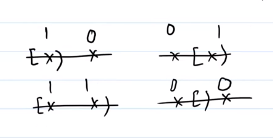
\includegraphics[scale=0.5]{bin strings.png}
    \label{fig:bin strings}
\end{center}

But can't shatter distinct $x_1 < x_2 < x_3$ since the binary string $\{ 1, 0, 1 \}$ can't be generated by our simple interval indicator class. So $VC(\F)=2$.

The lesson here is that despite being an infinite hypothesis class, $\F$ has a asymptotically sharp shattering coefficient bound.
\end{example}

Actually, we have the surprising result that shattering coefficients grow \emph{polynomially} with $n$, which is strongly constrasted with the trivial $2^n$ bound.

\begin{theorem}
[Sauer-Shelah]

Let $\F$ have finite VC dimension $d$. Then

\begin{equation}
    s(\F, n) \le \sum_{i=0}^d \binom{n}{i} \le (n+1)^d.
\end{equation}

\begin{proof}
\emph{Non-examinable}.

First pick any $x_{1:n}$. We claim that there are at least $|\F(x_{1:n})| - 1$ non-empty subsets of indices of $1:n$ such that $\F$ shatters these indices.

The result follows from this since we can specialise to the $x_{1:n}$ that achieves the shattering coefficient bound; where we'll have $|\F(x_{1:n})| = s(\F,n)$, and then the binomial coefficent falls out since we can't shatter any size $>d$ subsets by definition of VC dimension.

The claim is true since we can induct on $k := |\F(x_{1:n})|$ (note we may assume the result holds for any $n$ with this style of induction). The base case of size $k=1$ is vacuous. Assume we have the result for all $k'\le k$. We'll show we get the result with $k+1$.

The idea is that since we assumed way back that $|\F|\ge2$ always we can find an $x_j$ such that we can decompose $\F = \F_+ \sqcup \F_-$ (here, $\F = \F(x_{1:n})$ has size $k+1$) into non-empty subsets such that the first always classifies $x_j$ as 1, and the latter always as $-1$. Then the non-empty condition means we are now able to apply an induction procedure. We just do clever counting.

$|\F| = |\F_+| + |\F_-|$ and hence we have two positive integers summing to $k+1$ and hence the inductive hypothesis gives that the sets $\X_+$ and $\X_-$ of vectors shattered the two subsets have sizes summing to at least $k-1$ (we can't do better due to the $-1$ in hypothesis). Then for everything in the intersection of $\X_+$ and $\X_-$, we can add $x_j$ to these subsets of $x_{1:n}$ and get a genuinely new shattered vector. Finally the singleton $(x_j)$ can be shattered by the non-empty condition. We can put this together to get at least

\begin{equation}
    1 + |\X_+ \cap \X_-| + |\X_+ \cup \X_-| = |\X_+| + |\X_-| + 1 \ge (k-1) + 1 \ge k
\end{equation}

subsets shattered by $\F$. So we're done.

% such that we $|\F(x_{1:n})| = s(\F,n)$. Then we will claim that there are at least $|$
\end{proof}

\end{theorem}

\label{rademacher VC bound}

\begin{corollary}
\begin{equation}
    \R_n(\F) \le \sqrt{\frac{ 2 VC(\F) \log(n+1) }{n}} %todo sort out display of VC..
\end{equation}

(recall (\ref{empirical rad to combi}) and shattering definition).
\end{corollary}

%lecture 8

\begin{example}
Let $\X = \RR^p$ and consider the class $\F = \{ \one{A} \mid A \in \A \}$ where

\begin{equation}
    \A = \left\{ \prod_{j=1}^p ( - \infty, a_j ] \mid a_1, ... , a_p \in \RR \right\}.
\end{equation}

We claim that $VC(\F) = p$. 

After unpacking definitions, it is clear that we can shatter $n$ points.

It's slightly less easy to see that we can't shatter $p+1$ points. After checking the small cases for $n$, it's clear that we have some point which is not `extreme' in some direction (or at very least, is not \textit{uniquely} extreme in some direction). Then we can cook up a binary string with 0 in the place of this entry, and 1 everywhere else, and we can't get this behaviour.
\end{example}

\begin{theorem}
\label{VC dimension is dimension of sorts}
Let $\F$ be a vector space of functions. Then we can consider the class of classifiers $\H = \{ \text{sgn} \circ f \mid f \in \F \}$. Then

\begin{equation}
VC(\H) \le \dim \F. % the dimension of $\F$.
\end{equation}

\begin{proof}
We can first note that this generalises the previous result (I think I could cook up things to make this work with some zero product thing).

Let $d = \dim \F + 1$ and take $x_{1:d} \in \X^d$. We need show that $x_{1:d}$ cannot be shattered by $\H$.

Consider the linear map $L : \F \rightarrow \RR^d$ defined by $f \mapsto (f(x_1), ... , f(x_d))$. Then the image dimension is at most $d-1$ by rank-nullity. From here, take $\gamma \neq 0$ orthogonal to this image space. Then break $\gamma$ down in to its positive and non-negative components; let $\gamma_i > 0$ for all $i \in I_+$ and $\gamma_i < 0$ for all $i \in I_-$. Then

\begin{equation}
    \sum_{i \in I_+} \gamma_i f(x_i) + \sum_{i \in I_-} \gamma_i f(x_i) = 0
\label{gamma pos}
\end{equation}

holds for all $f \in \F$. Then the behaviour where $f(x_i) = \pm 1$ on $I_\pm$ cannot be observed since if so, the LHS of (\ref{gamma pos}) would be positive.
\end{proof}
\end{theorem}

\begin{example}
Consider $\X = [0,1)^2$ and $\F$ to be the set of polynomials of degree at most $d$, and define $\H$ as the set of signs of these polynomials as seen in (\ref{VC dimension is dimension of sorts}).

Then by stars and bars, $\dim \F = \binom{d+2}{2}$. So if $d=5$ then $VC(\H) \le 21$ and previous results (namely, (\ref{bound with rad}) and the VC bound (\ref{rademacher VC bound})) imply

\begin{equation}
    R(\hat{h}) - R(h^*) \le 2 \sqrt{\frac{2 \times 42 \log(n+1)}{n}} + \sqrt{\frac{2 \log (2/\delta)}{n}}.
\end{equation}

Comparing to the histogram classifier (\ref{the histogram classifier}), with the finite hypothesis class bound, we had

\begin{equation}
    R(\hat{h}) - R(h^*) \le \sqrt{\frac{2m^2 \log 2 + 2 \log (1 / \delta)}{n}} 
    % 2 \sqrt{\frac{2 \times 42 \log(n+1)}{n}} + \sqrt{\frac{2 \log (2/\delta)}{n}}.
\end{equation}

where *importantly*, the two $h^*$s are different: we're dealing with two different hypothesis classes.

with probability at least $1 - \delta$.
\end{example}    

and with that example over, we finish the most stats-heavy part of the course. Phew!

\section{Computation for ERM}

It turns out that the discontinuity of 0-1 loss means computation of the ERM is computationally intractable. We will therefore adjust our theory to work with \vocab{convex} loss functions that will still have values in $[0,M]$. This will mean that our result (\ref{ERM with rademacher}) will hold, although we will need to figure out what Rademacher complexity become with this new loss function.   % (even NP-hard in some scenarios?!).

% We will try and turn this hard problem into a convex optimisation problem. This will mean we wll

\subsection{Convex sets}

\begin{definition}
$C \subset \RR^d$ is \vocab{convex} if all lines segments lie entirely in $C$.
\end{definition}

\begin{example}
[Basic properties of convex sets]
Intersections of convex sets are themselves convex.
\end{example}

\begin{definition}
The \vocab{convex hull} of $S \subset \RR^d$, written $\conv S$ is the intersection of all convex sets containing $S$. By the above, it is unsurprisingly convex.
\end{definition}

\begin{definition}
$v \in \RR^d$ is a \vocab{convex combination} of $v_1, ... , v_m \in \RR^d$ if the $\alpha$ are non-negative and sum to 1 and

\begin{equation}
    v = \alpha_1 v_1 + ... + \alpha_m v_m.
\label{convex combination expression} 
\end{equation}
\end{definition}

\begin{lemma}
[Convex combinations ... are what you think they are]
For $S \subset \RR^d$, $v \in \conv S$ iff $v$ is a convex combination of some set of points in $S$.

\begin{proof}
Let $D$ be the set of all convex combinations of points from $S$.

Then $\conv S \subset D$ is on the example sheet.

To show $D \subset \conv S$ induct on the number $m$ of non-zero $\alpha$ terms appearing in  (\ref{convex combination expression}). The case $m=1$ is clear. Then for $m+1$ non-zero terms WLOG making the indices nice,

\begin{equation}
     v = \alpha_1 v_1 + ... + \alpha_{m+1} v_{m+1} = t \left(\frac{\alpha_1}{t} v_1 + ... + \frac{\alpha_m}{t} v_m\right) + (1-t) v_{m+1}.
\end{equation}

and terms here must indeed lie in $\conv S$ by its convexity.
% i.e as in the proof of the inclusion-exclusion formula, useeee
\end{proof}
\end{lemma}

\begin{theorem}
\label{linear convex lem}
Let $S \subset \RR^d$. For any linear map $L : \RR^d \rightarrow \RR^m$, $\conv L(S) = L(\conv S)$.

\begin{proof}
As before, intuitively clear. To formalise, use the convex combination characterisation and work both ways.
\end{proof}
\end{theorem}

\subsection{Convex functions}

We define (strictly) convex functions as we did in IB Optimisation.

\begin{definition}
Let $C \subset \RR^d$ be convex. Then $f : C \rightarrow \RR$ is \vocab{convex} if % $f$ sends points on the line segment joining two points in $C$ to a value less than the corresponding linear combination.  

\begin{equation}
    f(tx + (1-t)y) \le tf(x) + (1-t)f(y)
\end{equation}

$\forall t \in (0,1)$, and $x \neq y \in C$. $f$ is \emph{strictly convex} if the inequality is strict.
\end{definition}

\begin{example}
[Properties of convex functions]
Unsurprisingly, convex functions are closely related to convex sets. The following results are clear and/or on the second example sheet.
\begin{itemize}
    \item If $f$ is convex then $D = \{ x \in C \mid f(x) \le M \}$ is convex.
    \item The level sets of convex functions are convex sets.
    \item An important case of the first point is when the convex function is when applied to norm functions, which are always convex.
    \item If $f$ is $C^2$ then $f$ is convex iff its Hessian matrix is positive semi-definite. This is because of the supporting hyperplane (I think).
\end{itemize}
\end{example}

\begin{definition}
The \vocab{epigraph} of a convex function is the set of points 

\begin{equation}
    C = \{ (z,y) \in \RR^d \times \RR : y \ge f(z) \}.
\end{equation}
\label{epigraph}
\end{definition}

Why do we care about convex functions? It's because they allow \emph{global} properties to be deduced from \emph{local} properties; knowing $f(x)$ and $f(y)$ allows us to know a lot of things about all the values on the line segment joining $x$ and $y$. Local maxima will also be global maxima, obviously important for machine learning. % We saw in IB Optimisation that 

\subsection{Convex surrogates}

Consider $\H = \{ x \mapsto \sgn \beta^T x \mid \beta \in \RR^p \}$. To compute the ERM we need minimise (over $\beta$)

\begin{equation}
    \frac1n \sum_{i=1}^n \one{ Y_i \neq \sgn \beta^T X_i } \approx \frac1n \sum_{i=1}^n \one{Y_i \beta^T X_i \in (-\infty, 0]}
\end{equation}

where we have $\approx$ because of the annoying case where we defined $\sgn 0 = -1$.

If we replace the indicator function $\one{(-\infty, 0]}$ with a convex function, the resulting problem will become a convex optimisation problem.

Take the hypothesis class $\H$ to not be messy discontinuous functions but a family of real-valued functions. Then we could always recover a classifier post-composing with $\sgn$.

We shall consider losses of the form $\ell (h(x), y) = \phi (yh(x))$ where $\phi : \RR \rightarrow [0, \infty)$ is convex. The associated risk is called the \vocab{$\phi$-risk}. 

What shall we choose for $\phi$? Think about what properties are desirable. We are classifying correctly when $h(x)$ and $y$ have the same sign, and incorrectly classifying otherwise. This sort of situation is very similar to the setup for the barrier method in IB Optimisation.

Here are a few choices of $\phi$:

\begin{example}
[Convex surrogate loss functions]
All of the following loss functions are candidates for $\phi(h)$:

\begin{center}
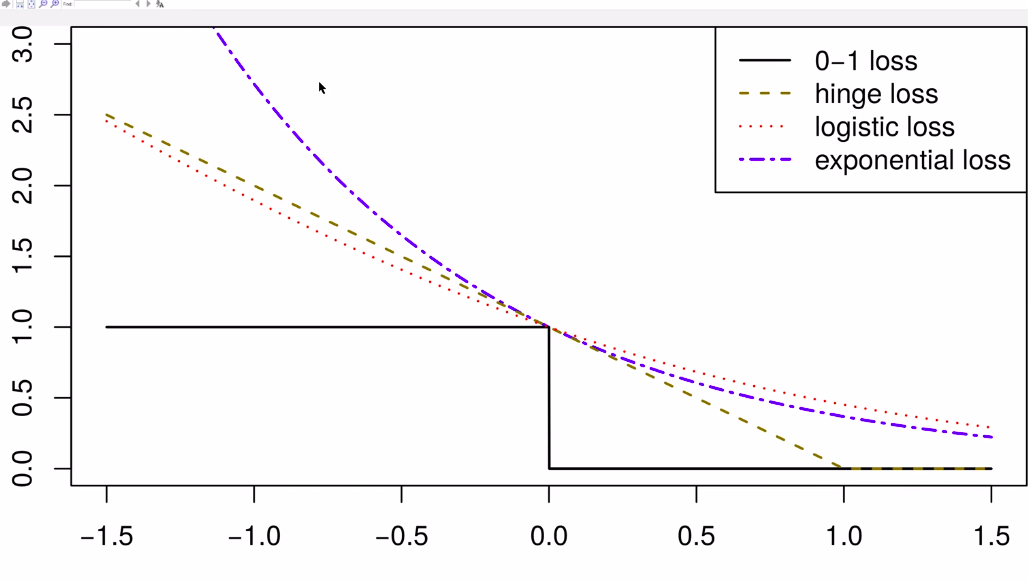
\includegraphics[scale=0.25]{surrogates1.png}
\label{surrogates picture}
\end{center}

\begin{itemize}
    \item Hinge loss $\max (1-h, 0)$
    \item Exponential loss $\exp -h  $
    \item Logistic loss $\log_2(1+e^{-h})$ 
    
    (where is 2 chosen so that logistic loss, like our original indicator take the value 1 at $h=0$)
\end{itemize}
\label{surrogates pic}
\end{example}

Let's prove that this is a good thing to do: that minimising $\phi$-risk minimises the true misclassification we want to minimise.

\begin{definition}
The \vocab{conditional $\phi$-risk} of $h$ is 
\begin{equation}
    \E{ \phi(Y h(X)) \mid X=x} 
\end{equation}
\end{definition}

Working much like we did in (\ref{not deep Bayes}),

\begin{align}
    \E{ \phi(Y h(X) \mid X=x} \\
    = \E{\phi(Y h(X) | X=x, Y=1} \eta(x) + \E{\phi(Y h(X) | X=x, Y=-1} (1 - \eta(x)) \\
    = \phi(h(x)) \eta(x) + \phi(-h(x))(1-\eta(x))
\end{align}

where $\eta(x) = \P{Y=1 \mid X=x}$.

For a generic $\eta \in [0,1]$ and $\alpha \in \RR$, let 

\begin{equation}
    C_\eta(\alpha) = \phi(\alpha) \eta + \phi(-\alpha)(1-\eta).
\end{equation}

% What are we trying to say here?

\begin{definition}
Say $\phi : \RR \rightarrow [0, \infty)$ is \vocab{classification calibrated} if $\forall \eta \in [0,1]$ with $\eta \neq 1/2$ (as before this was an annoying side case),

\begin{equation}
    \inf_{\alpha \in \RR} C_\eta(\alpha) < \inf_{\alpha : \alpha(2\eta - 1) \le 0} C_\eta (\alpha).
\end{equation}

This is dense, but it can be unpacked. We're working with this `generic' $\eta$ since we want to just study functions rather than have statistics and conditioning garbage going on. We call this property `calibrated' because what it is basically saying is that (ignoring the ambiguous `50-50' case) we incur a greater loss when we guess in contradiction to the Bayes classifier: this is the interpretation of the sign condition on the second $\inf$.
\end{definition}

% I think we're using these tools to prove the claim that our proxy goal of minimising $\phi$-risk is sufficient.
% So with these formalit

With these formalities we can turn engineering and rules of thumb (`which surrogate loss should I pick?') into maths:

\begin{theorem}
Let $\phi : \RR \rightarrow [0, \infty)$ be convex. Then if $\phi$ is differentiable at 0 and $\phi'(0)<0$, then $\phi$ is classification calibrated.

\begin{proof}
Since it's a composition of $\phi$ things, $C_\eta$ is convex and diffble at 0 with $C_\eta'(0) = (2\eta - 1)\phi'(0)$. Now separate into the cases $\eta > 1/2$, in which case $C_\eta'(0) < 0$. Then our picture is a `skewed parabola':

\begin{center}
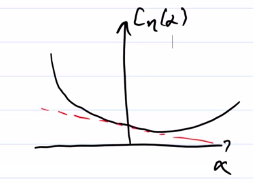
\includegraphics[scale=0.75]{skewparab.png}
\label{surrogates picture}
\end{center}

and the $\inf$ inequality should now be clear: all we need check is that we must get something smaller on the RHS than all of the LHS of $\alpha = 0$. But local diffbility means we must lie below $C_\eta(0)$ somewhere on the RHS, and by convexity on the LHS we must always lie above the tangent and hence above $C_\eta(0)$ too.

The other case is similar.
\end{proof}
\end{theorem}

%lecture 10

\subsection{Rademacher Complexity, Again}

Recall that our ERM work led to the result (\ref{ERM with rademacher}) that involved the Rademacher complexity $\R_n(\F)$.

In our setting now, we have $\F = \{ (x,y) \mapsto \phi( y h(x) ) \mid h \in \H \} $. We would like to relate $\R_n(\F)$ and $\R_n(\H)$.

\begin{lemma}
[The contraction lemma]
Suppose there exists some Lipschitz constant $L>0$ with

\begin{equation}
    |\phi(u) - \phi(u')| \le L|u-u'|.
\end{equation}

$\forall u, u' \in [-r,r]$ where $r = \sup h(x)$ (sup taken over all hypotheses and all inputs), since $y$ is always $\pm 1$ means these are the only values we'll ever evaluate $\phi$ at.

Then $\R_n (\F) \le L \R_n(\H)$.

\begin{proof}
\textit{Non-examinable}.

The two complexities in the inequality are the complexities of what our surrogate classification function spits out, and of the actual $\pm 1$ classifications.

This is a fairly long symbol pushing proof in the course notes. The important idea is that we need to turn $\frac1n \eps_i \phi(y_i h(x_i))$ terms into $\frac{L}{n}\eps_i h(x_i)$ terms. Let $i=1$ for ease of notation going forward.

Let $A : \H \times \{ -1, 1\}^{n-1}$ be a function that basically allows us to ignore the other $n-1$ terms. Then we can force into the scenario to use the Lipschitz bound as follows

\begin{align}
    \E{\sup_{h \in \H} \frac1n \eps_1 \phi(y_1h(x_1)) + A(h, \eps_{2:n}) \mid \eps_{2:n}} \\
    = \frac{1}{2n} \left( \sup_{h, g \in \H}{ \underbrace{\phi(y_1h(x_1)) - \phi(y_1g(x_1))}_{\le L |h(x_1) - g(x_1)|} + nA(h,\eps_{2:n}) + nA(g,\eps_{2:n})} \right)
\end{align}

and then considering what this absolute value means, we can accomplish the goal of turning $\frac1n \eps_i \phi(y_i h(x_i))$ terms into $\frac{L}{n}\eps_i h(x_i)$ terms, and we take expectation to clear the conditioning on $\eps_{2:n}$ and then repeat for the other $n-1$ terms.

% \begin{equation}
    % \sup_{h \in \H} 
% \end{equation}

\end{proof}
\end{lemma}

\begin{corollary}
\label{classic bound with phi}
Consider the setup of the contraction lemma and suppose $r < \infty$. Suppose that $\phi$ is non-increasing and let $M = \phi(-r)$. Then with probability at least $1 - \delta$, the ERM $\hat{h}$ of the $\phi$-risk satisfies 

\begin{equation}
\label{phi risk bound apapt}
    R_\phi(\hat{h}) - R_\phi(h^*) \le 2 L \R_n(\H) + M \sqrt{ 2 \log (2/\delta) / n }
\end{equation}
\end{corollary}

But is this even useful? For $\H = \{ x \mapsto x^T \beta \}$, $r$ and hence $M$\footnote{because we can make $\beta$ have large entries, whence $h(x)$ will grow large, and all such $\phi$ functions considered so far grow large as inputs grow large.} AND $\R_n(\H)$\footnote{This is true since the contraction lemma bounds by $\R_n(\F)$, and the definition of Rademacher complexity (\ref{Empirical rademacher conditioning}.) will have unbounded terms.} would not be finite, so we fail spectacularly to produce any meaningful result in two ways. However, it's clear things are going wrong since we're allowing $\beta$'s entries to get large. So, let's bound those entries.

\subsection{$\ell_2$ constraints}

Consider $\H = \{ x \mapsto x^T \beta : ||\beta||_2 \le \lambda \}$ and $\X = \{ x \in \RR^p : ||x||_2 \le C \}$, so by construction we resolve the $r=\infty$ issue; 

\begin{equation}
    \sup_{x \in \X, h \in \H} |h(x)| \le \lambda C 
\end{equation}

by Cauchy-Schwarz.

\begin{theorem}
[$\ell_2$-constrained Rademacher bound]
\label{L2 constrained rademacher bound}
For $x_{1:n} \in \X$ we have 

\begin{equation}
\hat{R}(\H(x_{1:n})) = \frac1n \E{ \sup_\beta \sum_{i=1}^n \eps_i x_i^T \beta } \le \frac{\lambda C}{\sqrt{n}}
\end{equation}

\begin{proof}
The summation is essentially a dot product, so actually let's use Cauchy-Schwarz once more

\begin{equation}
    \le \frac{\lambda}{n} \E{ \norm{ \sum_{i=1}^n \eps x_i }_2 }
\end{equation}

and now use Jensen on the square root function

\begin{equation}
    \le \frac{\lambda}{n} \left( \E{ \norm{ \sum_{i=1}^n \eps_i x_i }_2^2 } \right)^{1/2}
\end{equation}

and at this point many diagonal terms cancel (assuming we're really just squaring and ignoring the fancy norm) since $\E{\eps_i x_i^T x_j \eps_j} = 0$. Now the expectation will fall away:

\begin{equation}
    = \frac{\lambda}{n} \left( \sum_{i=1}^n \norm{x_i}_2^2 \right)^{1/2} \le \frac{ \lambda C }{\sqrt{n}}
\end{equation}
\end{proof}
\end{theorem}

\begin{example}
[Support vector machines]
\label{SVM theory}
Take $\phi$ to be hinge loss and $\H$ given by our $\ell_2$ constrained hypotheses we've been discussing.

Then this is a so-called support vector machine. We have from (\ref{classic bound with phi}) that with probability at least $1 - \delta$,

\begin{equation}
    R_\phi(\hat{h}) - R_\phi(h^*) \le \frac{2 \lambda C}{\sqrt{n}} + (\lambda C + 1) \sqrt{\frac{2 \log 2/\delta}{n}}.
\end{equation}
\end{example}

However, we only really care about misclassification risk. But

\begin{theorem}

In fact if $h^*$ minimises $\phi$ risk over $\H$ then

\begin{equation}
    R_\phi(\hat{h}) - R_\phi(h^*) \ge R(\sgn \circ \hat{h}) - R(\sgn \circ h^*)
\end{equation}

and further that $R(\sgn \circ h^*)$ is in fact the Bayes risk.

\begin{proof} % STILL TODO
Generalise from example sheet 2, question 11. %% @todo; hint is example sheet 2, question 11 for main result, and for the part involving Bayes risk somehow  is due to $\phi$ being classification calibrated.
\end{proof}
\end{theorem}

\subsection{Kernel machines (\textit{non-examinable})}

Consider a very general hypothesis class $\H = \{ \sum_{j=1}^d \phi_j(x) \beta_j \mid \beta \in \RR^d, \norm{\beta}_2 \le \lambda \}$ where $d \in \NN \cup \{ \infty \}$ (!). Surprisingly, the optimization problem is tractable. Consider the Lagrangian form of the objective

\begin{equation}
    \frac1n \sum_{i} \ell(h(X_i), Y_i) + \gamma \norm{\beta}_2^2
\end{equation}

where $\gamma$ is a Lagrange multiplier and $\Phi \in \RR^{n \times d}$ and $\Phi_{ij} = \phi_j(X_i)$. Note that $h(X_i) = (\Phi \beta)_i$. Introduce the projection matrix $P\in \RR^{d \times d}$ onto the \emph{row} space (not column space!) of $\Phi$. Then $\Phi \beta = \phi P \beta$. Also our norm decreases, since 

\begin{equation}
    \norm{\beta}_2^2 = \norm{P\beta}_2^2 + \norm{(I-P)\beta}_2^2
\end{equation}

which means WLOG we can consider only the $\beta$ must already lie in that row space. So $\hat{\beta} = \Phi^T \hat{\alpha}$ for some $\hat{\alpha} \in \RR^m$. Now let $k(x,x') = \sum_j \phi_j(x) \phi_j(x')$ and $K_{ij} = k(X_i,X_j)$ so that we have a \vocab{kernel} matrix $K = \Phi \Phi^T$. Then $\hat{\alpha}$ minimises (over $\alpha \in \RR^n$)

\begin{equation}
    \sum_{i=1}^n \ell((K\alpha)_i, Y_i) + \gamma \alpha^T K \alpha.
\end{equation}

This is an $n$-dimensional optimization problem!

The ERM $x \mapsto \sum_j \phi_j (x) \hat{\beta}_j$ is

\begin{equation} 
    \sum_j \phi_j (x) (\Phi^T \hat{\alpha})_j = \sum_j \phi_j(x) \sum_{i=1}^n \phi_j(X_i) \hat{\alpha}_i = \sum_i k(x, X_i) \hat{\alpha}_i.
\end{equation}

In fact the only place where the dimension $d$ even arises is in computing $\Phi$.

It turns out that for certain families of functions, the kernel $K$ can be computed fast (without potentially problematic sums over $d$ terms).

\begin{example}
[An example of where the $K$ computation is reasonable]

Suppose $\X= \RR^p$ where $p$
is large. Then if $d=p^2+p$,

\begin{equation}
    (\phi_1(x), ... , \phi_d(x)) = (x_1, ... , x_p, x_1x_1, x_1x_2, ... , x_1x_p, x_2x_1, ... , x_2x_p, ... , x_px_p)
\end{equation}

i.e. the first $p$ components are just the $x$ guys. Then the next $p^2$ components are all the pairwise products in lexicographic order.

Then in a nice way,

\begin{equation}
    k(x, x') = \sum_j x_j x_j' + \sum_j \sum_k x_j x_k x_j' x_k' = \left( \sum_j x_j x_j' + \frac12 \right)^2 - \frac14
\end{equation}
\end{example}

%lecture 11

Recall that our $\X = \{ x \in \RR^p : ||x||_2 \le C \}$. Since $C$ appears in several of the bounds (e.g. (\ref{L2 constrained rademacher bound})), we may hope that rescaling $C$ may be useful. However, this is not the case: we will need scale up the size of $\beta$ (perhaps because otherwise we're centred so close to 0 we will have very bad stability?) and hence the $\lambda C$ terms that appear in our inequalities won't be small.

It turns out that this situation arises in practise when our input data has a large number of features (equivalently, its dimension as a vector is large) and we expect that a low proportion of such features are useful. Then (I think!) scaling things won't fix our problems as all features will still be weighted in the same way.

\subsection{$\ell_1$ constraints}

\begin{definition}
The $\ell_1$ norm is 

\begin{equation}
    \norm{u}_1 = \sum_i |u_i|
\end{equation}

and the $\ell_\infty$ norm is

\begin{equation}
    \norm{u}_\infty = \max_i |u_i|.
\end{equation}
\end{definition}

Suppose that $\X = \{ x \in \RR^p : \norm{x}_\infty \le C \}$ and let $\H = \{ x \mapsto x^T \beta : ||\beta||_1 \le \lambda \}$. Then $x^T \beta \le C \lambda$. % why is there another inequality in lecture?!

\begin{lemma}
\label{es2 lemma}
For any set $A \subset \RR^n$, $\hat{\R}(A) = \hat{\R}(\conv A)$,

\begin{proof}
See example sheet 2. The notation here is a generalisation of the previous (\ref{empirical raddy}) definition; in that case we take the Rademacher complexity of $\F(z_{1:n})$ which is a set, so the definition naturally generalises.
\end{proof}
\end{lemma}

\begin{theorem}
\begin{equation}
    \{ \beta : \norm{\beta}_1 \le \lambda \} = \conv \left( S \right)
\end{equation}

where $S = \bigcup_{j=1}^p \{ \lambda e_j , - \lambda e_j  \}$.

\begin{proof}

Note that visually this is intuitive; 
\begin{center}
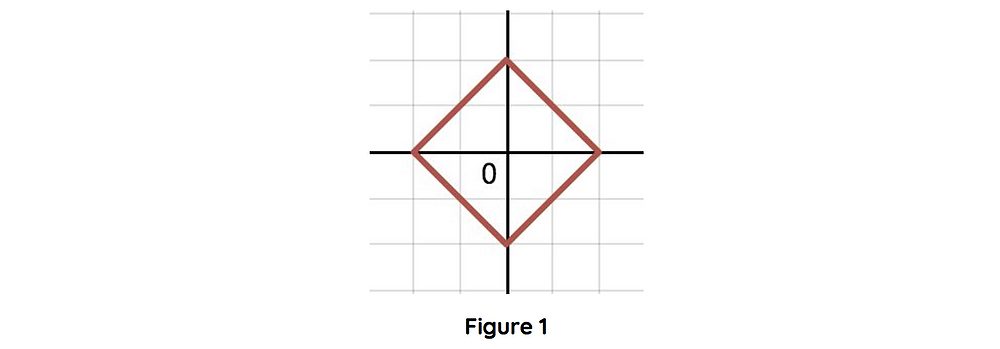
\includegraphics[scale=0.25]{tax2.png}
\label{surrogates picture}
\end{center}

we're saying that the interior of this shape is the convex hull of the four vertices.

Let's check the two cases: if $\beta$ is such that $\norm{\beta}_1 = \lambda$ then 

\begin{equation}
    \beta = \sum_{j=1}^p |\beta_j| \sgn (\beta_j) e_j = \sum_{j=1}^p \frac{|\beta_j|}{\lambda} \underbrace{( \lambda \sgn (\beta_j) e_j )}_{\in S}
\end{equation}

and since those coefficients are at most 1, indeed we get the result.

Next, if $\norm{\beta}_1 \le \lambda$, then rescale two copies of $\beta$ to have norm $\lambda$, and then take a linear combination of these points and use the prior case (for suitable $t_1$ and $t_2$):

\begin{equation}
    \beta = t_1 \frac{\lambda \beta}{ \normo{\beta}} + t_2 \left( \frac{-\lambda \beta}{\normo{\beta}} \right) \in \conv S.
\end{equation}
\end{proof}
\end{theorem}

Given $x_1, ... , x_n$, let $L:\RR^p \rightarrow \RR^n$ be the linear map given by

\begin{equation}
    L(\beta) = ( x_1^T\beta, ... , x_n^T\beta )^T,
\end{equation}

so we can write $\H(x_{1:n}) = L(\conv S) = \conv L(S)$ from (\ref{linear convex lem}), and then we can use (\ref{es2 lemma}):

\begin{equation}
    \hat{\R}(\H(x_{1:n})) = \hat{\R}(L(S)) = \frac{\lambda}{n} \E{ \max_{j=1}^p \left\lvert \sum_{i=1}^n \eps_i x_{ij} \right\rvert}
\end{equation}

where the second equality follows from the fact that we've reduced to the set $S$ which consists of just basis vectors (scaled by $\pm \lambda$).

Now each $\pm \sum_i \eps_i x_{ij}$ is sub-Gaussian with parameter

\begin{equation}
    \sqrt{ \sum_{i=1}^n x_{ij}^2 } \le C \sqrt{n}
\end{equation}

by (\ref{L3: linear combo subg}) and the fact that $\normi{x} \le C$. Now we can apply the max result (\ref{max subg upper bound}) with the following modification:

\begin{theorem}
[Adapting the $\max$ result for absolute values]

$\E{\max_{i=1}^n |W_i|} = \E{ \max(W_1, -W_1, W_2, -W_2, ... ,W_n,-W_n) } $ i.e itself the maximum of $2n$ terms.
\end{theorem}

namely

\begin{equation}
    \hat{R}(\H(x_{1:n})) \le \frac{\lambda}{n} \times C \sqrt{n} \times \sqrt{2 \log |S|} = \frac{\lambda C}{\sqrt{n}} \sqrt{2 \log (2p)}.
\end{equation}

where, alternatively, we can see the $2p$ arising as a consequence of our $S$ being defined with $\pm$ each coordinate.
 
% Also 

% \begin{equation}
%     \sup
% \end{equation}

\begin{example}
Take $\phi$ to be hinge loss and let $\H_1$ be the hypothesis class $\H = \{ x \mapsto x^T \beta : \normo{\beta} \le \lambda_1 \}$ and $\X = \{ -1, 1 \}^p$.

Then we can use (\ref{phi risk bound apapt}), and the risk gap bound turns out to be $O\left( \lambda_1 \sqrt{\frac{\log p}{n}} \right)$ (gory algebra omitted).

Due to our choice of $\X$, the bound for the corresponding $\ell_2$ constrained hypothesis class derived in (\ref{SVM theory}) is $O\left( \lambda_2 \sqrt{\frac{p}{n}} \right)$.

To compare these, Let $h_0$, identified with $\beta_0$, minimise $R_\phi$ over the set of hypotheses with unconstrained norm.

\begin{example}
If we assume that 

\begin{equation}
\beta_0 = \frac{1}{\sqrt{p}} (1,1,...,1)^T
\end{equation}

then for $h_0 \in \H_1$ to hold we need $\lambda_1 \ge \sqrt{p}$.

Hence we can't make the excess risk smaller than $O\left(\sqrt{\frac{p \log p}{n}} \right)$. % (wait, why? Doesn't the inequality direction mean this doesn't follow? Oh I suppose we can `bring lambda down' to the value of $\sqrt{p}$).

For $h_0 \in \H_2$ to hold we instead need $\lambda_2 \le 1$, in which case the risk bound is $O\left( \sqrt{\frac{p}{n}} \right)$.
\end{example}

\begin{example}
If instead

\begin{equation}
\beta_0 = \frac{1}{\sqrt{s}} (1,...,1,0,...,0)^T
\end{equation}

with $s$ non-zero entries, then the risk bounds are $O\left( \sqrt{\frac{s \log p}{n}} \right)$ and $O\left( \sqrt{\frac{p}{n}} \right)$, following through the same procedure.

Here, the $O\left( \sqrt{\frac{s \log p}{n}} \right)$ bound is the important one. This is because the form of $\beta_0$, `throwing away' most of the features, but still having very large dimension, then we actually have a really tight bound. The fact that we don't have the $s$ dependence in the $\ell_2$ means that $\ell_1$ constraints may be desirable in practise.

Still, if every feature is important, $\ell_2$ constrained hypothesis classes may perform better (even though the extra $\sqrt{\log p}$ seems negligible?).
\end{example}
\end{example}

\subsection{Projection onto convex sets}

Note that we've alluded to the fact that extremizing convex functions on convex sets is a computationally tractable problem. However, we haven't seen this explicitly. If we were to do gradient descent (from IB Optimization) in such a scenario what if after one step in the gradient's direction we were led to a point outside the convex set? We could move to the closest point in the convex set, doing \textit{projective} gradient descent. This could fail though, as for example $2$ is closest to $1$ in the convex set $(0,1)$ despite 1 not actually being in this set. So we may specialise to closed convex sets:

\begin{theorem}
Let $C \subset \RR^d$ be a closed convex set. Then for each $x \in \RR^d$, the minimiser $\pi_C(x)$ of $\normt{x-z}$ over $z\in C$ exists and is unique. We call $\pi_C(x)$ the \vocab{projection} of $x$ on $C$.

\begin{proof}
We can't immediately use tools from analysis to deduce that we achieve this value since while we are in a closed set, we're not necessarily in a bounded set so we might not have compactness. But actually, points far away will obviously not be the norm minimiser, so they don't matter. We can let $\mu = \inf_{z \in C} \normt{x-z}$ and then consider the compact $\bar{B}(x, \mu + 1) \cap C$. 

For uniqueness, we can use the \textit{strict} convexity of the function $x \mapsto \normt{x}^2$, and details are filled in on the example sheet.
\end{proof}
\end{theorem}

\begin{theorem}
\label{neggy convex thing}
In the notation of the previous result,
\begin{equation}
    (x - \pi_C(x))^T (z - \pi_C(x)) \le 0.
\end{equation}

\begin{proof}

After drawing a picture, this should be intuitive (the line segments meet at an obtuse angle).

\begin{center}
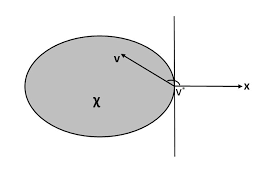
\includegraphics[scale=0.5]{proj.png}
\label{surrogates picture}
\end{center}

Formally, fix $x$, and let $\pi = \pi_C(x)$. If $z \in C$ then

\begin{equation}
    (1-t)\pi + tz \in C
\end{equation}

for all $t \in [0,1]$ by convexity definition. So

\begin{align}
    \normt{x-\pi}^2 \le \normt{x-\pi + t(\pi - z)}^2 \\
    = \normt{x-\pi}^2 - 2t(x-\pi)^T (z-\pi) + t^2 \normt{\pi-z}^2.
\end{align}

After rearranging, we can take $t \rightarrow 0^+$ and get the result.
\end{proof}
\label{proj negative}
\end{theorem}

\begin{theorem}
\label{projection is contraction}
$\pi_C$ is a \textit{contraction};

\begin{equation}
    \normt{\pi_C(x) - \pi_C(z)} \le \normt{x-z}
\end{equation}

for all $x,z \in \RR^d$.

\begin{proof}
Use (\ref{proj negative}) to note that 

\begin{equation}
    (x - \pi_C(x))^T (\pi_C(z) - \pi_C(x)) \le 0
\end{equation}

as well as 

\begin{equation}
    (\pi_C(z) - z)^T (\pi_C(z) - \pi_C(x)) \le 0
\end{equation}

(since $\pi_C(z)$ is its own projection onto the convex set). Adding these implies that

\begin{equation}
    \normt{\pi_C(x) - \pi_C(z)}^2 \le |(x-z)^T (\pi_C(x) - \pi_C(z))|
\end{equation}

now apply Cauchy-Schwarz:

\begin{align}
    \le \normt{x-z} \normt{\pi_C(x) - \pi_C(z)}.
\end{align}
\end{proof}

and divide through to deduce the result.
\end{theorem}

\subsection{Subgradients}
\label{subgradient_section}

What if the functions we want to apply gradient descent to functions that aren't differentiable? For example, hinge loss is not differentiable at $x=1$ (\ref{surrogates pic}).

Let's now introduce some terminology closely related to the supporting hyperplane theorem:

\begin{definition}
$g \in \RR^d$ is a \vocab{subgradient} of a convex function $f : \RR^d \rightarrow \RR$ at $x \in \RR^d$ if

\begin{equation}
    f(z) - f(x) \ge g^T (z-x)
\end{equation}

for all $z \in \RR^d$. We call the set of all such $g$ the \vocab{subgradient}, denoted $\partial f(x)$.
\end{definition}

% i.e. this is a word for the possible parameters for a supporting hyperplane at $x$.

\begin{example}
% [Application to SVMs (see () too)]
The hinge loss $\phi(u) = \max(0,1-u)$ has $\partial \phi(1) = [-1,0]$:

\begin{center}
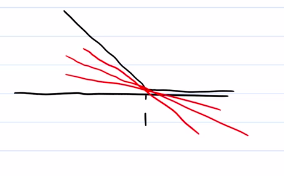
\includegraphics[scale=0.5]{hinge subdiff.png}
\label{hinge subdiffs}
\end{center}
\end{example}

\begin{theorem}
If $f : \RR^d \rightarrow \RR$ is convex, then $\partial f(x)$ is non-empty for all $x \in \RR^d$.
\begin{proof}
Non-examinable.

There is intuition that, actually, if our convex function is not differentiable then it will be easier rather than harder to find a supporting hyperplane; example (\ref{hinge subdiffs}) showed that the sub-differential set was a whole interval rather than just a point.

We shall generalise the idea used in proving Jensen's inequality from IA Probability, where we took the $\sup$ of the gradients of the chords joining $(x,f(x))$ to a point on its left, and the $\inf$ of the gradients of the chords joining it to a point on its right.

Let $C$ be $f$'s epigraph (\ref{epigraph}). Then take a sequence 

\begin{equation}
    w_1, w_2, ... \in \RR^{d+1} \setminus C
\end{equation}

such that $w_k \rightarrow (x,f(x))$. Then we can use (\ref{neggy convex thing}) to find a $v_k$ with $\normt{v_k}=1$ such that

\begin{equation}
    v_k^T w \le v_k^T w_k
\end{equation}

for all $w \in C$. For example, a rescaled $w_k - \pi_C(w_k)$ works. Then the $v_k$ lie in a compact unit ball, so by Bolzano-Weierstrass find a convergent subsequence that converges to some $v = (v_1, v_2)$ where $v_1 \in \RR^d$ and $v_2 \in \RR$. So

\begin{equation}
v_1^T z + v_2 y \le v_1^T x + v_2 f(x)    
\end{equation}

for all $(z,y) \in C$. Setting $z=x$ and growing $y$ to be larger than $f(x)$, we get that $v_2 \le 0$. $z$ being unconstrained (in $\RR^d$) means that $v_2 \neq 0$ either.

So after dividing through by $v_2$ and rearranging, $v_2/v_1$ is in $\partial f(x)$.
\end{proof}
\end{theorem}

\begin{theorem}
$f$ differentiable implies that $\partial f(x) = \{ \nabla f(x) \}$.

\begin{proof}
Like most of this section, this is intuitively obvious in two dimensions, and we need to symbol push to generalise to higher dimensions.

Let $g \in \RR^d$ be the subgradient. Then we have, for any $z \in \RR^d$

\begin{equation}
    \nabla f(x)^T z = \lim_{t \downarrow 0} \frac{ f(x+tz)-f(x) }{ t } \ge g^T z
\end{equation}

where the inequality follows from subgradient definition.

But taking $z = g - \nabla f(x)$ we get that $\normt{\nabla f(x) - g}^2 \le 0$ and hence the result.
\end{proof}
\end{theorem}

\begin{theorem}
[Subgradient calculus]
\label{subgrad calc}
Let $f,f_1,f_2 : \RR^d \rightarrow \RR$ be convex. Then
\begin{enumerate}
    \item $\partial(\alpha f)(x) = \{ \alpha g : g \in \partial f(x) \}$ for $\alpha>0$.
    \item Suppose that $h:\RR^m \rightarrow \RR$ is a composition $h = f \circ g$ where $g$ is an affine function possibly from one dimension to another). Then $\partial h(x) = A^T \partial f(Ax+b) $
    \item $\partial(f_1 + f_2)(x) = \{ g_1 + g_2 : g_1 \in \partial f_1(x), g_2 \in \partial f_2(x) \}$
\end{enumerate}
\begin{proof}
1) and 2) are immediate from writing out definitions.

For 3), we first prove the 1D case. This relies on the following characterisation
\end{proof}
\end{theorem}

\begin{example}
[SVMs continued (see also (\ref{SVM theory}))]
\label{SVM subgs}
Consider % the objective function

\begin{equation}
    f(\beta) = \frac1n \sum_{i=1}^n \max(1 - y_i x_i^T \beta, 0).
\end{equation}

Let $\phi(u) = \max(1-u,0)$. Then combining (\ref{hinge subdiffs}) with $u>1$ and $u<1$ (where $\phi$ is differentiable, we can use (\ref{subgrad calc}) to decompose $f(\beta)$:

Write 

\begin{equation}
    h_i(\beta) = \max(1-y_i x_i^T \beta)
\end{equation}

so $\partial h_i(\beta) = \{ -y_i x_i t : t \in [0,1] \}$ when $y_i x_i^T \beta = 1$. From the second two properties now,
\begin{equation}
    \partial f (\beta) = -\frac1n \sum_{i=1}^n y_i x_i t_i
\end{equation}
where the range of each of the $t_i$s is either the singleton sets $\{ -1 \}$ or $\{ 0 \}$ if $y_i x_i^T \beta \neq 1$, or else the interval $[0,1]$.
\end{example}

\subsection{Gradient Descent}

Suppose we're solving the optimization problem

\begin{equation}
    \min_{\beta \in C} f(\beta)
\end{equation}

where $C$ is closed and convex.

Let $\beta_1 \in C$ be an initial guess and $k \in \NN$ be the number of steps, and the sequence of positive step sizes $(\eta_s)_{s=1}^{k-1}$. Then the gradient descent algorithm is the following:

\begin{algorithmic}
% $\beta_1 \in C$, $k \in \NN$, $(\eta_s)_{s=1}^{k-1}$
\For{$s = 1, ... , k-1$}
    \State $g_s \gets \partial f(\beta_s)$ \Comment{Set to \textit{any} subgradient}
    \State $z_{s+1} \gets \beta_s - \eta_s g_s$
    \State $\beta_{s+1} \gets \pi_C(z_{s+1})$
\EndFor

\Return $\bar{\beta} = \frac{1}{k} \sum_{s=1}^k \beta_s$ \Comment{An average over all steps, NOT $\beta_s$}
\label{gradient descent algo}
\end{algorithmic}

\begin{remark}$\bar{\beta} \in C$ by convexity.
\end{remark} %todo fix corrections thing landing here

\begin{remark}The choice to return this average of $\beta$ values rather than $\beta_s$ may not be too unlike that choice; it is likely the gradients will decrease in size as we optimize, and hence the $\beta_i$ will cluster around $\beta_s$.\end{remark}

\begin{theorem}
\label{maths with gradient descent algo}
Suppose $\hat{\beta}$ is a minimiser of a convex function $f:\RR^p \rightarrow \RR$ over a closed convex set $C \subset \RR^p$, playing a very similar role to the ERMs we've worked so much with. 

Suppose we have two boundedness assumptions $\sup_{\beta \in C} \norm{\beta} \le R < \infty$ and $\sup_{\beta \in C} \sup_{g \in \partial f(\beta)} \normt{g} \le L < \infty$. Then if $\eta_s \equiv \eta = 2R / L\sqrt{k}$ the output $\bar{\beta}$ of the gradient descent algorithm above satisfies

\begin{equation}
    f(\bar{\beta}) - f(\hat{\beta}) \le \frac{2LR}{\sqrt{k}}.
\label{our classic bounding thing for grad descent algo}
\end{equation}

\begin{proof}
$f(\beta) \ge f(\beta_s) + g_s^T(\beta-\beta_s)$ for all $\beta$, so 
\begin{align}
f(\beta_s) - f(\hat{\beta}) \le g_s^T (\beta_s - \hat{\beta}) = \frac{1}{\eta} (\beta_s - z_{s+1})^T (\beta_s - \hat{\beta}) \\
= \frac{1}{2\eta} \left (\normt{\hat{\beta} - \beta_s}^2 + \normt{z_{s+1}-\beta_s}^2 - \normt{\hat{\beta} - z_{s+1}}^2 \right) \\
\end{align}

(see (\ref{gradient descent algo}) for definitions) for the first equality, and the second inequality is a sort of polarisation identity. Now use projection-is-contraction result (\ref{projection is contraction}) to note that $\normt{z_{s+1} - \hat{\beta}}^2 \ge \normt{\pi_C(z_{s+1}) - \pi_C( \hat{ \beta })}^2  = \normt{\beta_{s+1} - \hat{\beta}}^2$, so now we can apply our Lipschitz-like subgradient $L$ bound:

\begin{equation}
    f(\beta_s) - f(\hat{\beta}) \le \frac{1}{2 \eta} \left( \eta^2 \underbrace{\normt{g_s}^2}_{\le L^2} + \normt{\hat{\beta} - \beta_s}^2 - \normt{\hat{\beta} - \beta_{s+1}}^2 \right)
\end{equation}

and thus when we sum this quantity, we magically get telescoping: % (what about '$\beta_{s+2}$'?):

\begin{align}
\frac{1}{k} \sum_{s=1}^k f(\beta_s) - f(\hat{\beta}) \le \frac{\eta L^2}{2} + \frac{\normt{\hat{\beta} - \beta_1}^2 - \normt{\hat{\beta} - \beta_{k+1}}^2}{2\eta k} \\
\le \frac{\eta L^2}{2} + \frac{2R^2}{\eta k}
\end{align}

since $\max_{x,y \in C} \normt{x-y}^2 = 4R^2$, and we just ignore that minus term.

Now the $\eta = 2R / L\sqrt{k}$ choice in fact is the minimiser, and by Jensen's,

\begin{equation}
    \frac1k \sum_s f(\beta_s) \le f(\bar{\beta})
\end{equation}

and hence the result follows.
\end{proof}
\end{theorem}

\begin{remark}
In general, $t^* = \argmin_t \frac{A}{t} + \frac{t}{B}$ satisfies $\frac{A}{t^*} = \frac{t^*}{B}$.
\end{remark}

\begin{example}
[SVMs again]
In the notation continued from (\ref{SVM subgs}) we say the subgradients at some $\beta$ were of the form

\begin{equation}
    g = \frac1n \sum_{i=1}^n y_i x_i t_i
\end{equation}

where we had $|t_i| \le 1$. So by the triangle inequality we have the subgradient bound

\begin{equation}
    \normt{g}^2 \le C
\end{equation}

where $C$ is the $\ell_2$ norm bound for the $x \in \X$.

So application of the last result gives the bound

\begin{equation}
    f(\bar{\beta}) - f(\hat{\beta}) \le 2C\lambda / \sqrt{k}
\end{equation}

where $\lambda$ is the bound on the $\beta$ in the hypothesis class.
\end{example}

\begin{example}
[Mandatory COVID Example (!)]
Gradient descent is a more general method than a tool for ERM.

We have data on initial cases from Wuhan, and specifically the time $B$ when they entered Wuhan, the time $E$ when they left Wuhan, and the time when symptoms began $S$. Suppose each person was infected with COVID at time $T$. Then of course the incubation period $S-T$ is a very important thing we need to calculate! In this case, we may care to what extent $S-T$ depends on individuals' factors.

The negative log likelihood (of each probability that the incubation period is $n$ days) is a convex function, and so we have formally setup applying gradient descent to a linear model.

Applying this to men and women who contracted COVID and plotting a CDF, we see that the incubation period for women (in \color{blue}{blue}\color{black}) and the men (\color{red}{red}\color{black}) are different; in fact it is statistically significant that system onset is more likely to be very early or very late for men; this variance is large. However on average the incubation period is similar between the genders.

Of course, this is the `real world' so cultural differences could account for this, as men may be more likely to report symptoms earlier etc.
\begin{center}
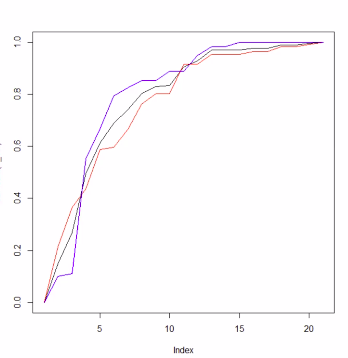
\includegraphics[scale=0.5]{men wamen.png}
    \label{fig:men wamen covid}
\end{center}

\end{example}

\subsection{Stochastic Gradient Descent}

In general a significant computational bottleneck on applying gradient descent is computing the (sub)gradient, as for example even in ERM it will be the sum of $n$ terms where $n$ is large.

\vocab{Stochastic gradient descent} (SGD) can circumvent this issue in the case of minimising convex functions of the form

\begin{equation}
    f(\beta) = \E{ \tilde{f} (\beta; U)}
\end{equation}

where $\tilde{f} : \RR^p \times \U \rightarrow \RR$ is such that $\beta \mapsto \tilde{f} (\beta; U)$ is convex for all $u \in \U$, and $U$ is a random variable taking values in $\U$.

\begin{example}
This setup encompasses ERM: let $U$ be distributed uniformly on $\{ 1, ... , n \}$. Then the ERM objective function with $\H = \{ h_\beta : \beta \in C \}$ can be written as 

\begin{equation}
    \frac1n \sum_{i=1}^n \ell(h_\beta(x_i), y_i) = \E{ \ell(h_\beta(x_U), y_U)} = \E{\tilde{f} (\beta; U)} 
\end{equation}

so long as our training data is fixed. The only randomness is in $U$.
\end{example}

Written in pseudocode, using the same input data as (\ref{gradient descent algo}) in addition to several i.i.d. copies $U_1, ... , U_{k-1}$ of $U$.

\begin{algorithmic}
% $\beta_1 \in C$, $k \in \NN$, $(\eta_s)_{s=1}^{k-1}$
\For{$s = 1, ... , k-1$}
    \State $\tilde{g}_s \gets \partial f(\beta_s; U_s)$ \Comment{See remark (\ref{subg rema})}
    \State $z_{s+1} \gets \beta_s - \eta_s \tilde{g}_s$
    \State $\beta_{s+1} \gets \pi_C(z_{s+1})$
\EndFor

\Return $\bar{\beta} = \frac{1}{k} \sum_{s=1}^k \beta_s$ \Comment{An average over all steps, NOT $\beta_s$}
\label{SGD gradient descent algo}
\end{algorithmic}

\begin{remark}
\label{subg rema}
The subgradient $\partial \tilde{f}$ is taken with respect to $\beta_s$ \textit{only}: we `fix' the $U_s$ things in $\tilde{f}(\beta; U_s)$ first.
\end{remark}

\begin{remark}
This is pretty much the same as (\ref{gradient descent algo}) except we now have tildes, and of course $f$ is different.
\end{remark}

\begin{theorem}
Suppose $\hat{\beta}$ is a minimiser of $f$ as above over a closed convex set $C \subset \RR^p$. 

Suppose that we have the same bound $\sup_{\beta \in C} \normt{\beta} \le R < \infty$ and same $\eta_s \equiv \eta = 2R / L\sqrt{k}$ condition as we had before for the not-stochastic case (\ref{maths with gradient descent algo}) and that we have a slightly different subgradient bound:

\begin{equation}
    \sup_{\beta \in C} \E{\sup_{\tilde{g} \in \partial \tilde{f} (\beta_i; U)} \normt{\tilde{g}}^2} \le L^2 < \infty.
\end{equation}

that involves squaring, since this is actually how we used the bound last time, and we can't avoid this since $\E{X^2} \neq \E{X}^2$.

Then the output $\bar{\beta}$ of the gradient descent algorithm above satisfies an analogous result to (\ref{our classic bounding thing for grad descent algo}) but with expectations:

\begin{equation}
    \E{f(\bar{\beta}) - f(\hat{\beta})} \le \frac{2LR}{\sqrt{k}}.
% \label{our classic bounding thing for 
\end{equation}

\begin{proof}
% The difficulty of applying the sam
This is not the same as (\ref{maths with gradient descent algo}) since we won't get telescoping due to the changing $U_s$ guys. So as ever, we sneakily use conditional expectation by defining

\begin{equation}
    g_s = \E{\tilde{g}_s \mid \beta_s}.
\end{equation}

$U_s$ is independent of $\beta_s$ (because $\beta_s$ is computed from $U_{s-1}$) so the following manipulation works

\begin{equation}
    \E{ \tilde{f}(\beta;U_s) \mid \beta_s } = \E{\tilde{f}(\beta;U_s)} = f(\beta) \ge f(\beta_s) + g_s^T (\beta - \beta_s)
\end{equation}

for all $\beta$, so $g \in \partial f(\beta_s)$. So we can insert $\tilde{g}$ as follows

\begin{equation}
    f(\beta_s) - f(\hat{\beta}) \le g_s^T (\beta_s - \hat{\beta}) = \E{\tilde{g}_s^T (\beta - \hat{\beta}) \mid \beta_s}
\end{equation}

and now we can use the same (polarisation-like) manipulations from (\ref{maths with gradient descent algo}), where everything will be surrounded with $\E{... \mid \beta_s}$. We get that the above is

\begin{align}
    \le \frac{1}{2\eta} \E{ \eta^2 \normt{\tilde{g}_s}^2 + \normt{\hat{\beta} - \beta_s}^2 - \normt{\hat{\beta} - \beta_{s+1}}^2 \mid \beta_s}
\end{align}

now use the tower property to bring that expectation down, and then we will get telescoping:

\begin{equation}
    \E{\frac1n \sum_{s=1}^k f(\beta_s)} - f(\hat{\beta}) \le \frac{\eta L^2}{2} + \frac{\normt{\beta_1 - \hat{\beta}}^2}{2 \eta k} \le \frac{2LR}{\sqrt{k}}.
\end{equation}

and once plugging in our $\eta$ choice and using Jensen's finishes this.

% Then in fact this lies in $\partial f (\beta_s)$; indeed, 

% \begin{equation}
    % \tilde{f} (\beta; U_s) \ge \tilde{f} (\beta_s;U_s) + \tilde{g}_s^T (\beta - \beta_s)
% \end{equation}
\end{proof}
\end{theorem}

\section{Popular Machine Learning Methods}

In this section

How do we choose the $\lambda$ constraining our e.g. $\ell_2$-constrained hypothesis class? This is a case where we want to consider multiple different machine learning methods, i.e. each $\lambda$ gives rise to a different method.

This leads to \vocab{cross-validation}, which is the biggest take-away from the course.

\begin{definition}
A \vocab{machine learning method} is a function

\begin{equation}
    H : D \rightarrow \RR^{\X}
\end{equation}

where $D$ is the training data, i.e. a machine learning method takes as input the training data $D = (X_i, Y_i)_{i=1}^n$ and outputs a hypothesis $H_D : \X \rightarrow \RR$.
\end{definition}

Let $H^1, ... , H^m$ be a collection of machine learning methods. Ideally, we would choose the `best' method $H^j$, where

\begin{equation}
    \E{ \ell (H_D^j(X), Y) \mid D }
\label{hard target}
\end{equation}

where this expectation is taken over essentially a `new' independent sample from $\X \times \Y$. This is intractable generally since we only `see' $D$ (i.e. see everything we've done on ERM!).

An easier approach is to try to minimise the expectation of (\ref{hard target}):

\begin{equation}
    \E{ \E{ \ell (H_D^j(X), Y) \mid D } }.
\label{easier cross validation target}
\end{equation}

\begin{definition}
\vocab{Cross-validation} is the process of splitting the dataset $D$ into $v$ \vocab{folds} $A_1, ... , A_v$ that partition $D$.

Define $D_{-k} = D \setminus A_k$, and $H_{-k}^j=H_{D-k}^j$.
\end{definition}

\begin{definition}
The cross-validation error $\CV$ is defined as

\begin{equation}
    \CV(j) = \frac1n \sum_{k=1}^v \sum_{i \in A_k} \ell(H^j_{-k}(X_i), Y_i)
\end{equation}
\label{cv def}
\end{definition}

\begin{remark}
(\ref{cv def}) is a (usually upwards) biased estimate of (\ref{easier cross validation target}), because we have a factor of $\frac1n$ and $n - |A_k| < n$.
\end{remark}

\begin{remark}
$v=n$ corresponds to \vocab{leave-one-out-cross-validation} which gives the least bias, but can have high variance as the summand in (\ref{cv def}) will tend to be positively correlated (Why is this exclusive to $v=n$, and why does the implication follow?).
\end{remark}

\subsection{Adaboost}

Given a base set $\B$ of `base' classifiers $h : \X \rightarrow \{ -1, +1 \}$ with the property 

\begin{equation}
h \in \B \implies -h \in \B,
\label{properr}
\end{equation}

consider the class

\begin{equation}
    \H = \left\{ \sum_{m=1}^M \beta_m h_m : \beta_m \in \RR, h_m \in \B, 1 \le m \le M  \right\}
\end{equation}

$M$ is called the \vocab{tuning parameter} which corresponds to .

\vocab{Adaboost} can be
motivated as a greedy ERM over $\H$ using exponential loss.

Setting $\hat{f}_0$ to be the zero function $x \mapsto 0$ as our `initial guess' at a hypothesis, adaboost performs the following update for each step $1 \le m \le M$:

\begin{align}
    (\hat{\beta}_m, \hat{h}_m) = \argmin_{\beta \ge 0 , h \in \B} \frac1n \sum_{i=1}^n \exp{ -Y_i \{ \hat{f}_{m-1} (X_i) + \beta h(X_i) \} } \\
    \hat{f}_m = \hat{f}_{m-1} + \hat{\beta}_m \hat{h}_m
\label{adaboost update}
\end{align}

where property (\ref{properr}) allows us to only need consider $\beta \ge 0$.

The final classification is performed according to $\sgn \circ \hat{f}_M$.

\begin{remark}
As mentioned, this is a greedy \textit{algorithm}, it is quite unlike the previous ERM procedures that generally guarentee some sort of minimization.
\end{remark}

To make this process implementable, we can separate the process of the $h$ and $\beta$ updates as follows:

\begin{equation}
    w_i^{(m)} = \frac1n \exp{ -Y_i \hat{f}_{m-1}(X_i) }.
\end{equation}

Then the expression we take an $\argmin$ over in (\ref{adaboost update}) is, decomposing,

\begin{align}
    e^\beta \sum_{i=1}^n w_i^{(m)} \one{ h(X_i) = Y_i } + e^{-\beta} \sum_{i=1}^n w_i^{(m)} \one{h(X_i) \neq Y_i} \\
    (e^\beta - e^{-\beta}) \sum_{i=1}^n w_i^{(m)} \one{h(X_i) \neq Y_i} +  e^{-\beta} \sum_{i=1}^n w_i^{(m)}.
\label{dwrtb}
\end{align}

Now this motivates us to define a `weighted error'

\begin{equation}
    \err_m(h) = \frac{\sum_{i=1}^n w_i^{(m)} \one{h(X_i) \neq Y_i}}{\sum_{i=1}^n w_i^{(m)}}.
\label{errdef}
\end{equation}

which is defined assuming that no $h \in \beta$ perfectly classifies the data. This setup allows us to rewrite the $h$ update in (\ref{adaboost update}) as

\begin{equation}
   \hat{h}_m = \argmin_{h \in \B} \err_m(h)
\end{equation}

Note that this reduction of the minimisation problem relies centrally on the $e^{\beta} - e^{-\beta}$ term in (\ref{dwrtb}) being positive, which is fine since we have property (\ref{properr}).

Now we can just consider this new $ \hat{h}_m$ as fixed, and differentiating (\ref{dwrtb}) with respect to $\beta$ in order to get the expression for the updated $\beta$ as follows:

\begin{equation}
    \hat{\beta}_m = \frac12 \log \left( \frac{1 - \err_m(\hat{h}_m)}{\err_m(\hat{h}_m)} \right).
\end{equation}

\begin{example}
[Adaboost applied to decision stumps]

\label{decision stumps}

Let $\X = \RR^p$ and consider the class of \vocab{decision stumps}

\begin{equation}
\B = \{ h_{a,j,1}(x) = \sgn(x_j-a),  h_{a,j,2}(x) = \sgn(a-x_j) : a \in \RR, 1 \le j \le p \}.
\end{equation}

i.e. the set of basic classifiers that pick a coordinate, and a parameter, and classify based on what side of that parameter we fall.

% These are known as 'stumps' since essentially this always moves us left or right, and so we have a `stump' at $a$.

To perform adaboost, finding the optimal weights $w_1, ... , w_n > 0$ (omitting superscript $m$), for each $1 \le j \le p$, first sort $\{ X_{ij} \}_{i=1}^n$ assuming distinctness: $X_{(1)j} < ... < X_{(n)j}$. %For a fixed $j$, assume that $X_{(i)j} = X_{ij} = x_i$.

Now fixing $j$, WLOG assume that $X_{(i)j} = X_{ij} = x_i$. Now 

\begin{equation}
    \err(h_{x_{k+1}, j, 1}) - \err(h_{x_{k}, j, 1}) = \frac{Y_{k+1}w_{k+1}}{\sum_l w_l}.
\end{equation}

by referring to (\ref{errdef}), and noting that having sorted anything, moving our parameter just slightly to the right will only change one classification (and increase or decrease the error, depending on the sign of $Y_i$).

So to pick the optimal $h_{a,j,1}$ (over variable $a$), we need consider a bunch of cumulative sums, and something similar happens with $h_{a,j,2}$. We can sort the $X$ before performing adaboost, and hence after preprocessing the complexity of the algorithm is $O(np)$.
\end{example}

\begin{remark}
The original $\H$ is uncountable, but it turns out the only $a$ values that we care about (as the resulting classifier will behave the same on the training data) are the values inbetween coordinates $X_{ij}$ in the finite input $D$ which consists of only $np$ values total.
\end{remark}

This same strategy of taking a simple set of hypotheses and then `boosting' them into a better hypothesis is more general than adaboost.

\subsection{Gradient Boosting}

This technique is used widely e.g. in most winning entries to kaggle competitions.

It can be motivated by the following thought experiment: consider applying gradient descent directly in order to minimise the risk $R(h)= \E{\ell(h(X), Y)}$ (over all function $h$). This would involve the following steps:

\begin{itemize}
    \item Have an initial guess $f_0 : \X \rightarrow \RR$.
    \item For each $m=1,...,M$ compute
    \begin{align}
        g_m(x) = \frac{\partial \E{\ell(\theta, Y) | X=x}}{\partial \theta} \bigg\vert_{f_{m-1}(x)} \\
        = \E{\frac{\partial \ell (\theta , Y)}{\partial \theta} \bigg\vert_{f_{m-1}(x)} \bigg\vert X=x}
        \label{x function}
    \end{align}
    where we make suitable regularity conditions to exchange $\partial$ and $\E{ ... }$.
    \item Update $f_m = f_{m-1} - \eta g_m$ where $\eta > 0$ is a small step length.
 \end{itemize}

But this is, as ever in the course, idealized since the expectation is over the distribution of $Y$. 

Now recall from (\ref{best least squares}) that (\ref{x function}) (thought of as a function of $x$) is the minimiser of

\begin{equation}
    \E{\left( \frac{\partial \ell (\theta , Y)}{\partial \theta} \bigg\vert_{f_{m-1}(X)} - f(X) \right)^2}
\label{gradient boosting least squares}
\end{equation} %todo maybe email about changing this

over all functions $f : \X \rightarrow \RR$. This is the motivation for \vocab{gradient boosting} where we empirically minimise (\ref{gradient boosting least squares}) using a regression approach.

\begin{definition}
Let $H$ be a base regression method that takes as its argument training data $D$ and outputs a hypothesis $H_D : \X \rightarrow \RR$. $\
ell$ the loss may be any type of loss (including a convex surrogate).

Then \vocab{gradient boosting} takes as input the data $X_{1:n}$ and $Y_{1:n}$ as well as $\eta > 0$, $H$ and $M$ and

\begin{equation}
    \hat{\mu} = \argmin_{\mu \in \RR} \frac1n \sum_{i=1}^n \ell(\mu, Y_i).
\end{equation}

We set $f_0(x) = \hat{\mu}$, i.e we initially guess the best constant function (with respect to the data, and the loss function).

The idea of the algorithm is to use our base regression procedure itself to generate a `gradient hypothesis' $\hat{g}(m)$ at each stage of the algorithm that is intended to be a close approximation of $f$ in (\ref{gradient boosting least squares}). This will therefore be an empirical approximation of the `true' gradient (\ref{x function}).

\begin{algorithmic}
\For{$m = 1, ... , M$}
    \State $W_i \gets \frac{\partial}{\partial \theta} \ell (\theta, Y_i) \mid_{\theta = \hat{f}_{m-1}(X_i)}$ \Comment{One gradient per item of training data.}
    % \State $z_{s+1} \gets \beta_s - \eta_s \tilde{g}_s$
    \State $\hat{g}_m \gets H_{(X_{1:n}, W_{1:n})}$ \Comment{i.e. apply our method $H$.}
    \State $\hat{f}_m \gets \hat{f}_{m-1} - \eta \hat{g}_m$
    % \State $\beta_{s+1} \gets \pi_C(z_{s+1})$
\EndFor

\Return $\hat{f}_M$ \Comment{Possibly composed with $\sgn$ in the classification setting.} % $\bar{\beta} = \frac{1}{k} \sum_{s=1}^k \beta_s$ \Comment{An average over all steps, NOT $\beta_s$}
% \label{SGD gradient descent algo}
\label{gradient boosting}

\end{algorithmic}
\end{definition}

\subsection{Decision Trees}

Gradient boosting is particularly effective at optimising `decision tree methods' that are generalisations of the decision tree stumps (\ref{decision stumps}).

Firstly let's get an example of what a decision tree is:

\begin{example}
[Decision tree by example, not formality]

Suppose we are in a $0-1$ classification setting and wish to recursively draw decision boundaries based on the decision boundaries that maximise the reduction in least squares error. Restricting to horizontal and vertical lines only, we get a plot that has a bunch of nested regions:

\begin{center}
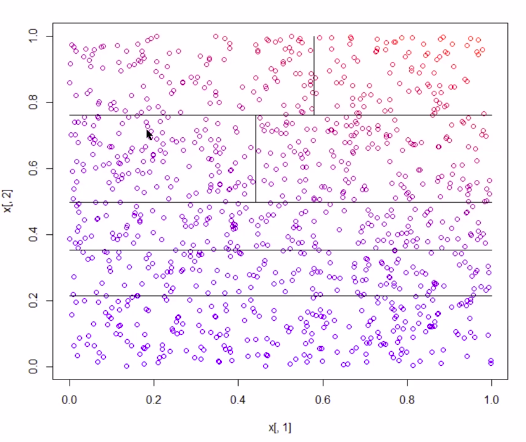
\includegraphics[scale=0.5]{multiple boundaries.png}
    % \label{fig:bin strings}
\end{center}

It is computationally efficient to compute such boundaries due to the reduction in size of each region with each iteration.

The method is called a decision tree procedure since there are several ways to visualize our resultant classifier, and one of them is a decision tree (think 'if-else' statement in code), at the bottom left:

\begin{center}
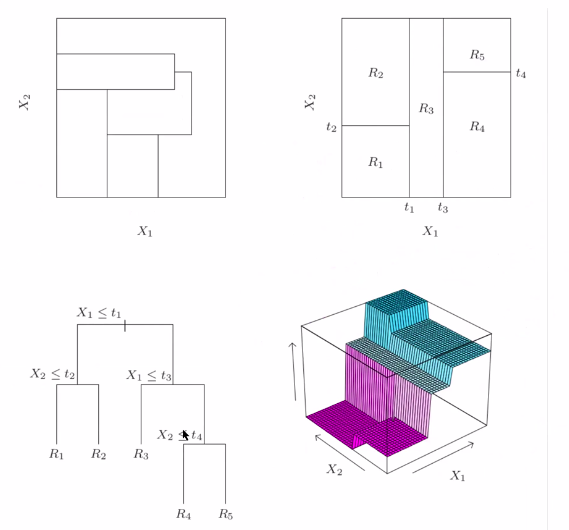
\includegraphics[scale=0.25]{why decision tree.png}
    \label{fig:bin strings}
\end{center}
\end{example}

Formally, 

\begin{definition}
Given data $(X_1, Y_1), ... , (X_n, Y_n)$, a \vocab{decision tree} performs the following:

\begin{enumerate}
    \item Take as input the maximum number of regions $J$. Initialize $\hat{\R} = \{ \RR^p \}$.
    
    \item For each region $R \in \hat{\R}$ such that $I = \{ i : X_i \in R \}$ has $|I| > 1$ perform the following:
    
    \begin{itemize}
            \item For each $j = 1, ... , p$ let $S_j$ be the set of midpoints between adjacent $\{ X_{ij} \}_{i \in I}$ (i.e specialise to one coordinate then sort points in $R$ by this coordinate and extract the midpoints).
            
            \item Find the predictor $\hat{j}_R$ and the split point $\hat{s}_R$ to minimise the residual sum of squares drop
            
            \begin{equation}
                \min_{c_1 \in \RR} \underbrace{\sum_{i \in I : X_{ij} \le s} (Y_i - c_1)^2 + \min_{c_2 \in \RR} \sum_{i \in I : X_{ij} > s} (Y_i - c_2)^2 }_{\text{The residual sum of squares when we split at $s$}} - \underbrace{\min_{c \in \RR} \sum_{i \in I} (Y_i - c)^2}_{\text{RSS before the split}}.
            \label{RSS drop}
            \end{equation}
            
            where the last, pre-split term does not affect the optimization but is included for our analysis to come.
    \end{itemize}

\item Let $\hat{R}$ be the region yielding the lowest value of the drop in RSS, and update our partition $\hat{\R}$ accordingly (unenlightening symbols omitted).

\item Repeat steps 2 and 3 until $|\hat{\R}|=J$.

\item Writing $\hat{\R} = \{ \hat{R}_1, ... , \hat{R}_J \}$, let $\hat{I}_j = \{ i : X_i \in \hat{R}_j \}$ and 

\begin{equation}
    \hat{\gamma}_j = \frac{1}{|\hat{I}_j|} \sum_{i \in \hat{I}_j} Y_i.
\end{equation}

i.e. a weighted average of the results of things in region.

\item Return the classifier $\hat{T} : \RR^p \rightarrow \RR$ that classifies based on the plurality of the region that data points fall into:

\begin{equation}
    \hat{T}(x) = \sum_{j=1}^J \hat{\gamma}_j \one{x \in \hat{R}_j}.
\end{equation}

\end{enumerate}
\end{definition}

%final lecture

% \begin{example}
% [Application of gradient boosting to decision trees]

% Suppose that we are using squared error loss. Then the $W_i$ terms in (\ref{gradient boosting}) are $-2(Y_i - \hat{f}_{m-1}(X_i))$, a `negative residual' as such.

% Then the update rule very explicitly
% \end{example}

\subsection{Random Forests}

Consider the regression setting (i.e where $Y_i \in \RR$) with squared error loss. Let $\hat{T}_D$ be a decision tree trained on iid data $D = (X_i, Y_i)_{i=1}^n$. Let $\bar{T}(x) = \E{\hat{T}_D(x)}$.

\begin{remark}
Here, we consider the training data to be random, hence the expectation with the argument $x$.
\end{remark}

Let $(X,Y)$ be independent of $D$ and distributed like the training data. Recall the expectation decomposition (\ref{best least squares}), then we can compute

\begin{align}
    \E{R(\hat{T}_D)} = \E{ (Y - \DT(x))^2 } \\
    = \E{(Y- \underbrace{\E{Y \mid X, D}}_
    {\E{Y|X}})^2} + \E{ (\E{Y|X} - \DT(X))^2 } 
\end{align}

Use the tower property, and fudge in $\bar{T}(X)$ noting that $\bar{T} = \E{\DT}$ (so cross-terms disappear) to write

\begin{align}
    \E{\E{(Y-\E{Y \mid X})^2} | X} + \E{\left(\DT - \E{\DT}\right)^2} + \E{(\bar{T} - \E{Y|X})^2}
\end{align} 

both these first two terms are now conditional variances:

\begin{align}
    = \underbrace{\E{\text{Var} (Y|X) }}_ {\text{`Irreducible error', tree independent}} + \underbrace{\E{\text{Var} (\DT | X)}}_{\text{Variance of the tree}} + \underbrace{\E{ (\bar{T} - \E{Y|X})^2 }}_{\text{Squared bias}}.
\end{align}

As we increase the number of regions, while the squared bias will reduce, However, the variance of the tree will tend to increase due the $\gamma$ coefficients in the decision tree construction being far more variable.

\begin{definition}
A \vocab{random forest} procedure samples from the data $D$ with replacement in order to form datasets $D_1^*, ... , D_B^*$. It then fits trees $\hat{T}^{(b)}$ to the data $D_b^*$, but when searching for the best variable to split upon, restrict ourselves to a random sample of $m_{\text{try}}$ of the $p$ predictors.

Then we average out the trees: we output $f_{\text{rf}} = \frac1B \sum_{b=1}^B \hat{T}^{(b)}$.
\end{definition}

What is the reason for this sampling procedure? For one thing, it may reduce the computational complexity. It also makes the $\hat{T}^{(b)}$ more independent.

If for $b_1 \neq b_2$ and some $x \in \RR^p$ we have that $\text{Corr}(\hat{T}^{(b_1)}(x), \hat{T}^{(b_2)}(x))= \rho \ge 0$ then when can directly compute the forest variance via the formula,

\begin{equation}
    \text{Var}(f_{\text{rf}}) = \left(  \rho + \frac{1-\rho}{B} \right) \text{Var}(\hat{T}^{(1)}(x))
\end{equation}

so we can't expect increasing $B$ alone decreasing the forest variance; we also need decrease $\rho$. This can be done by choosing a small $m_\text{try}$ since this will increase likelihood that the individual forests come from different classifiers. But then squared bias would (probably...) increase.

\subsection{Neural Networks}

This will be the last machine learning technique in the course, and we focus only on feed-forward neural networks, the state-of-the-art for many problems.

Neural networks for classification problems are based around a class of hypotheses $\H$, that is rich in that it is consists of many function compositions.

\begin{definition}
A \vocab{neural network} is based around a set of hypotheses $h(x)$ defined by 

\begin{equation}
    h(x) = A^{(d)} \circ g \circ A^{(d-1)} \circ g \circ ... \circ A^{(1)}(x)
\end{equation}

where $d$ is the depth of the neural network, $A^{(k)} : \RR^{m_k} \rightarrow \RR^{m_{k+1}}$ is an affine function $A(v) = \beta^{(k)} v + \mu^{(k)}$, and $g : \RR^m \rightarrow \RR^m$ is a non-linear activation function that acts component-wise by a function $\psi(u)$. Some popular choices include $\text{ReLU}(x) = \max(x,0)$ and $\sigma(x) = 1/(1+e^{-u})$. % that possibly changes
\end{definition}

\begin{remark}
If $g$ was not non-linear, the whole function would collapse into a single affine function!
\end{remark}

Let's set up some definitions in order to show how we can apply SGD to such hypotheses:

\begin{definition}
$h^{(0)} = x$ is the input layer to the neural network, $x^{(k)} := A^{(k)}(h^{(k-1)})$, the \vocab{hidden layers} of the network are given by $h^{(k)} = g(x^{(k)})$ for $k<d$ and the output (layer) is $x^{(d)} = h(x)$.
\end{definition}

Further terminology is that the vector input to $h$ is called the `input layer', the output $g \circ A^{(i)} \circ g \circ ... \circ A^{(1)}(x)$ at each stage is called the `hidden layer' output, and the final output is called the output layer. The terminology is used as each component can be thought of as a nodes in a graph, with edges all edges between nodes in adjacent layers.

The process of training a neural network is the process of applying SGD to the parameters $(\beta,\mu)$ of all the affine functions, with surrogate loss $\phi$. This turns out to be computationally tractable:

\subsubsection{Back-Propagation}

We let $z = \phi(yh(x)) = \phi(y x^{(d)})$ be our loss. Then initially compute

\begin{equation}
    \frac{\partial z}{\partial x^{(d)}} = y \phi ' (yx^{(d)}).
\label{first bit neural}
\end{equation}

Recall that our output $x^{(d)}$ is a function of the last hidden layer which is a simple affine function, so

\begin{align}
    \frac{\partial z}{\partial \beta_{1k}^{(d)}} = \frac{\partial z}{\partial x^{(d)}} h_k^{(d-1)}, \\
    \frac{\partial z}{\partial \mu^{(d)}} = \frac{\partial z}{\partial x^{(d)}}.
\end{align}

by differentiating the affine function expression $A = \beta x + \mu$.

Now we can propagate further backwards by writing

\begin{equation}
    \frac{\partial z}{\partial h_j^{(d-1)}} = \frac{\partial z}{\partial x^{(d)}} \beta_{1j}^{(d)}
\end{equation}

and then passing through the affine function

\begin{equation}
    \frac{\partial z}{\partial x_j^{(d-1)}} = \frac{\partial z}{\partial j_j^{d-1}} \psi ' (x_j^{(d-1)}).
\end{equation}

And now we're back to a $\frac{\partial z}{\partial x}$ expression as in (\ref{first bit neural}), so we can do this all again to get the gradients with respect to all the parameters further back in the network.

\begin{remark}
A much lighter introduction (which is slower paced!) can be found at \url{http://neuralnetworksanddeeplearning.com}. Thie author implements a neural network in basic python, while (importantly for mathmos!) explaining the choices made in both the design of the neural net architecture, and implementation choices.

\begin{center}
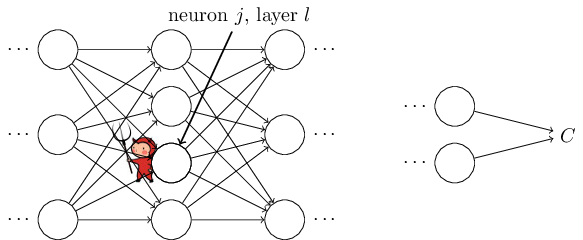
\includegraphics[scale=0.5]{demon2.png}
    \label{fig:demon}
% \caption{From 
\end{center}

\end{remark}

\begin{thebibliography}{9}
\bibitem{Course Notes}
Rajen D. Shah (2021), \emph{Mathematics of Machine Learning}, \url{http://www.statslab.cam.ac.uk/~rds37/teaching/machine_learning/notes.pdf}.

\bibitem{MIT Notes}
Philippe Rigollet, \emph{18.657: Mathematics of Machine Learning}, \url{https://ocw.mit.edu/courses/mathematics/18-657-mathematics-of-machine-learning-fall-2015/lecture-notes/MIT18_657F15_LecNote.pdf}.

\bibitem{HoeffdingExercise}
Ecole Normale Superieure.
\emph{FIFMA - Statistique 2020-2021.}
Available at \url{arthurconmy.github.io/assets/MML/HoeffdingExercise.pdf}.

\bibitem{FrenchDudeConditional}
Unknown source (linked on a French mathematician's blog).
\emph{Conditional Expectation}
Available at \url{arthurconmy.github.io/assets/MML/ConditionalExpectation.pdf}
\end{thebibliography}
\end{document}